% Lines starting with a percent sign (%) are comments. LaTeX will 
% not process those lines. Similarly, everything after a percent 
% sign in a line is considered a comment. To produce a percent sign
% in the output, write \% (backslash followed by the percent sign). 
% ==================================================================
% Usage instructions:
% ------------------------------------------------------------------
% The file is heavily commented so that you know what the various
% commands do. Feel free to remove any comments you don't need from
% your own copy. When redistributing the example thesis file, please
% retain all the comments for the benefit of other thesis writers! 
% ==================================================================
% Compilation instructions: 
% ------------------------------------------------------------------
% Use pdflatex to compile! Input images are expected as PDF files.
% Example compilation:
% ------------------------------------------------------------------
% > pdflatex thesis-example.tex
% > bibtex thesis-example
% > pdflatex thesis-example.tex
% > pdflatex thesis-example.tex
% ------------------------------------------------------------------
% You need to run pdflatex multiple times so that all the cross-references
% are fixed. pdflatex will tell you if you need to re-run it (a warning
% will be issued)  
% ------------------------------------------------------------------
% Compilation has been tested to work in ukk.cs.hut.fi and kosh.hut.fi
% - if you have problems of missing .sty -files, then the local LaTeX
% environment does not have all the required packages installed.
% For example, when compiling in vipunen.hut.fi, you get an error that
% tikz.sty is missing - in this case you must either compile somewhere
% else, or you cannot use sTikZ graphics in your thesis and must therefore
% remove or comment out the tikz package and all the tikz definitions. 
% ------------------------------------------------------------------

% General information
% ==================================================================
% Package documentation:
% 
% The comments often refer to package documentation. (Almost) all LaTeX
% packages have documentation accompanying them, so you can read the
% package documentation for further information. When a package 'xxx' is
% installed to your local LaTeX environment (the document compiles
% when you have \usepackage{xxx} and LaTeX does not complain), you can 
% find the documentation somewhere in the local LaTeX texmf directory
% hierarchy. In ukk.cs.hut.fi, this is /usr/texlive/2008/texmf-dist,
% and the documentation for the titlesec package (for example) can be 
% found at /usr/texlive/2008/texmf-dist/doc/latex/titlesec/titlesec.pdf.
% Most often the documentation is located as a PDF file in 
% /usr/texlive/2008/texmf-dist/doc/latex/xxx, where xxx is the package name; 
% however, documentation for TikZ is in
% /usr/texlive/2008/texmf-dist/doc/latex/generic/pgf/pgfmanual.pdf
% (this is because TikZ is a front-end for PGF, which is meant to be a 
% generic portable graphics format for LaTeX).
% You can try to look for the package manual using the ``find'' shell
% command in Linux machines; the find databases are up-to-date at least
% in ukk.cs.hut.fi. Just type ``find xxx'', where xxx is the package
% name, and you should find a documentation file.
% Note that in some packages, the documentation is in the DVI file
% format. In this case, you can copy the DVI file to your home directory,
% and convert it to PDF with the dvipdfm command (or you can read the
% DVI file directly with a DVI viewer).
% 
% If you can't find the documentation for a package, just try Googling
% for ``latex packagename''; most often you can get a direct link to the
% package manual in PDF format.
% ------------------------------------------------------------------


% Document class for the thesis is report
% ------------------------------------------------------------------
% You can change this but do so at your own risk - it may break other things.
% Note that the option pdftext is used for pdflatex; there is no
% pdflatex option. 
% ------------------------------------------------------------------
\documentclass[12pt,a4paper,oneside,pdftex]{report}

% The input files (tex files) are encoded with the latin-1 encoding 
% (ISO-8859-1 works). Change the latin1-option if you use UTF8 
% (at some point LaTeX did not work with UTF8, but I'm not sure
% what the current situation is) 
\usepackage[utf8]{inputenc}
% OT1 font encoding seems to work better than T1. Check the rendered
% PDF file to see if the fonts are encoded properly as vectors (instead
% of rendered bitmaps). You can do this by zooming very close to any letter 
% - if the letter is shown pixelated, you should change this setting 
% (try commenting out the entire line, for example).  
\usepackage[OT1]{fontenc}
% The babel package provides hyphenating instructions for LaTeX. Give
% the languages you wish to use in your thesis as options to the babel
% package (as shown below). You can remove any language you are not
% going to use.
% Examples of valid language codes: english (or USenglish), british, 
% finnish, swedish; and so on.
\usepackage[english]{babel}


% Font selection
% ------------------------------------------------------------------
% The default LaTeX font is a very good font for rendering your 
% thesis. It is a very professional font, which will always be 
% accepted. 
% If you, however, wish to spicen up your thesis, you can try out
% these font variants by uncommenting one of the following lines
% (or by finding another font package). The fonts shown here are 
% all fonts that you could use in your thesis (not too silly). 
% Changing the font causes the layouts to shift a bit; you many
% need to manually adjust some layouts. Check the warning messages
% LaTeX gives you.
% ------------------------------------------------------------------
% To find another font, check out the font catalogue from
% http://www.tug.dk/FontCatalogue/mathfonts.html
% This link points to the list of fonts that support maths, but
% that's a fairly important point for master's theses.
% ------------------------------------------------------------------
% <rant>
% Remember, there is no excuse to use Comic Sans, ever, in any
% situation! (Well, maybe in speech bubbles in comics, but there 
% are better options for those too)
% </rant>

% \usepackage{palatino}
% \usepackage{tgpagella}



% Optional packages
% ------------------------------------------------------------------
% Select those packages that you need for your thesis. You may delete
% or comment the rest.

% Natbib allows you to select the format of the bibliography references.
% The first example uses numbered citations: 
\usepackage[square,sort&compress,numbers]{natbib}
% The second example uses author-year citations.
% If you use author-year citations, change the bibliography style (below); 
% acm style does not work with author-year citations.
% Also, you should use \citet (cite in text) when you wish to refer
% to the author directly (\citet{blaablaa} said blaa blaa), and 
% \citep when you wish to refer similarly than with numbered citations
% (It has been said that blaa blaa~\citep{blaablaa}).
% \usepackage[square]{natbib}

% The alltt package provides an all-teletype environment that acts
% like verbatim but you can use LaTeX commands in it. Uncomment if 
% you want to use this environment. 
% \usepackage{alltt}

% The eurosym package provides a euro symbol. Use with \euro{}
\usepackage{eurosym} 

% Verbatim provides a standard teletype environment that renderes
% the text exactly as written in the tex file. Useful for code
% snippets (although you can also use the listings package to get
% automatic code formatting). 
\usepackage{verbatim}

% The listing package provides automatic code formatting utilities
% so that you can copy-paste code examples and have them rendered
% nicely. See the package documentation for details.
% \usepackage{listings}

% The fancuvrb package provides fancier verbatim environments 
% (you can, for example, put borders around the verbatim text area
% and so on). See package for details.
% \usepackage{fancyvrb}

% Supertabular provides a tabular environment that can span multiple 
% pages. 
%\usepackage{supertabular}
% Longtable provides a tabular environment that can span multiple 
% pages. This is used in the example acronyms file. 
\usepackage{longtable}

% The fancyhdr package allows you to set your the page headers 
% manually, and allows you to add separator lines and so on. 
% Check the package documentation. 
% \usepackage{fancyhdr}

% Subfigure package allows you to use subfigures (i.e. many subfigures
% within one figure environment). These can have different labels and
% they are numbered automatically. Check the package documentation. 
% \usepackage{subfigure}

% The titlesec package can be used to alter the look of the titles 
% of sections, chapters, and so on. This example uses the ``medium'' 
% package option which sets the titles to a medium size, making them
% a bit smaller than what is the default. You can fine-tune the 
% title fonts and sizes by using the package options. See the package
% documentation.
\usepackage[medium]{titlesec}

% The TikZ package allows you to create professional technical figures.
% The learning curve is quite steep, but it is definitely worth it if 
% you wish to have really good-looking technical figures. 
\usepackage{tikz}
% You also need to specify which TikZ libraries you use
\usetikzlibrary{positioning}
\usetikzlibrary{calc}
\usetikzlibrary{arrows}
\usetikzlibrary{decorations.pathmorphing,decorations.markings}
\usetikzlibrary{shapes}
\usetikzlibrary{patterns}

\usepackage{amssymb}
\usepackage{amsmath}
\usepackage{booktabs}
\usepackage{tabularx}
\usepackage{adjustbox}
\usepackage[ruled]{algorithm2e}
\usepackage{amsthm}
\usepackage{thmtools}
\usepackage{caption}
\usepackage{subcaption}
\usepackage{url}

\declaretheorem[style=plain,numberwithin=section]{theorem}
\declaretheorem[style=plain,sibling=theorem]{lemma}
\declaretheorem[style=plain,sibling=theorem]{proposition}
\declaretheorem[style=plain,sibling=theorem]{corollary}
\declaretheorem[style=plain,sibling=theorem]{claim}
\declaretheorem[style=plain,sibling=theorem]{observation}


\declaretheorem[style=definition,sibling=theorem]{definition}
\declaretheorem[style=definition,sibling=theorem]{conjecture}
\declaretheorem[style=definition,sibling=theorem]{example}
\declaretheorem[style=definition,sibling=theorem]{problem}

\declaretheorem[style=remark,sibling=theorem]{remark}




% The aalto-thesis package provides typesetting instructions for the
% standard master's thesis parts (abstracts, front page, and so on)
% Load this package second-to-last, just before the hyperref package.
% Options that you can use: 
%   mydraft - renders the thesis in draft mode. 
%             Do not use for the final version. 
%   doublenumbering - [optional] number the first pages of the thesis
%                     with roman numerals (i, ii, iii, ...); and start
%                     arabic numbering (1, 2, 3, ...) only on the 
%                     first page of the first chapter
%   twoinstructors  - changes the title of instructors to plural form
%   twosupervisors  - changes the title of supervisors to plural form
% \usepackage[mydraft]{aalto-thesis}
%\usepackage[mydraft,doublenumbering]{aalto-thesis}
\usepackage{aalto-thesis}


\renewcommand{\algorithmautorefname}{Algorithm} % so algorithm is capitalized when using autoref


% Hyperref
% ------------------------------------------------------------------
% Hyperref creates links from URLs, for references, and creates a
% TOC in the PDF file.
% This package must be the last one you include, because it has
% compatibility issues with many other packages and it fixes
% those issues when it is loaded.   
%\RequirePackage[pdftex]{hyperref}
\RequirePackage[pdfa]{hyperref}
% Setup hyperref so that links are clickable but do not look 
% different
\hypersetup{colorlinks=false,raiselinks=false,breaklinks=true}
\hypersetup{pdfborder={0 0 0}}
\hypersetup{bookmarksnumbered=true}
% The following line suggests the PDF reader that it should show the 
% first level of bookmarks opened in the hierarchical bookmark view. 
\hypersetup{bookmarksopen=true,bookmarksopenlevel=1}
% Hyperref can also set up the PDF metadata fields. These are
% set a bit later on, after the thesis setup.   


% Thesis setup
% ==================================================================
% Change these to fit your own thesis.
% \COMMAND always refers to the English version;
% \FCOMMAND refers to the Finnish version; and
% \SCOMMAND refers to the Swedish version.
% You may comment/remove those language variants that you do not use
% (but then you must not include the abstracts for that language)
% ------------------------------------------------------------------
% If you do not find the command for a text that is shown in the cover page or
% in the abstract texts, check the aalto-thesis.sty file and locate the text
% from there. 
% All the texts are configured in language-specific blocks (lots of commands
% that look like this: \renewcommand{\ATCITY}{Espoo}.
% You can just fix the texts there. Just remember to check all the language
% variants you use (they are all there in the same place). 
% ------------------------------------------------------------------
\newcommand{\TITLE}{Automated classification of distributed graph problems}
\newcommand{\FTITLE}{Ohjelmistoprosessit m�nteille:}
\newcommand{\STITLE}{Den stora stygga vargen:}
\newcommand{\SUBTITLE}{}
\newcommand{\FSUBTITLE}{Uusi organisaatio, uudet py�r�t}
\newcommand{\SSUBTITLE}{Lilla Vargens universum}
\newcommand{\DATE}{April 21, 2021}
\newcommand{\FDATE}{14. helmikuuta 2018}
\newcommand{\SDATE}{Den 18 februari 2018}

% Supervisors and instructors
% ------------------------------------------------------------------
% Usually thesis have one supervisor and one advisor. Sometimes you
% may have two advisors and, in double degree
% programs, you may have two supervisors. 
% If you have two supervisors, write both names here, separate them with a 
% double-backslash (see below for an example)
% Also remember to add the package option ``twosupervisors'' or
% ``twoinstructors'' to the aalto-thesis package (aalto-thesis.sty
% file line 72), so that the titles are in plural.
% Example of one supervisor:
%\newcommand{\SUPERVISOR}{Professor Antti Yl�-J��ski}
%\newcommand{\FSUPERVISOR}{Professori Antti Yl�-J��ski}
%\newcommand{\SSUPERVISOR}{Professor Antti Yl�-J��ski}
% Example of twosupervisors:
\newcommand{\SUPERVISOR}{Professor Jukka Suomela}
\newcommand{\FSUPERVISOR}{Professori Jukka Suomela}
\newcommand{\SSUPERVISOR}{Professor Jukka Suomela}

% If you have only one instructor, just write one name here
\newcommand{\INSTRUCTOR}{Professor Jukka Suomela}
\newcommand{\FINSTRUCTOR}{Diplomi-insinööri Oili Ohjaaja}
\newcommand{\SINSTRUCTOR}{Diplomingenjör Oili Ohjaaja}
% If you have two instructors, separate them with \\ to create linefeeds
% \newcommand{\INSTRUCTOR}{Oili Ohjaaja M.Sc. (Tech.)\\
%  Elli Opas M.Sc. (Tech)}
%\newcommand{\FINSTRUCTOR}{Diplomi-insin��ri Oili Ohjaaja\\
%  Diplomi-insin��ri Elli Opas}
%\newcommand{\SINSTRUCTOR}{Diplomingenj�r Oili Ohjaaja\\
%  Diplomingenj�r Elli Opas}

% If you have two supervisors, it is common to write the schools
% of the supervisors in the cover page. If the following command is defined,
% then the supervisor names shown here are printed in the cover page. Otherwise,
% the supervisor names defined above are used.
% \newcommand{\COVERSUPERVISOR}{Professor Jukka Suomela, Aalto University}

% The same option is for the instructors, if you have multiple instructors.
% \newcommand{\COVERINSTRUCTOR}{Oili Ohjaaja M.Sc. (Tech.), Aalto University\\
%  Elli Opas M.Sc. (Tech), Aalto SCI}


% Other stuff
% ------------------------------------------------------------------
\newcommand{\PROFESSORSHIP}{Computer Science}
\newcommand{\FPROFESSORSHIP}{Tietotekniikka}
\newcommand{\SPROFESSORSHIP}{Datateknik}
% Professorship code is the same in all languages
\newcommand{\PROFCODE}{SCI3042}
\newcommand{\KEYWORDS}{distributed algorithms, distributed computing, locally checkable labeling problems,
round elimination, graph algorithms}
\newcommand{\FKEYWORDS}{aineistot, aitta, akustiikka, Alankomaat,
aluerakentaminen, aapinen, ankka, aasinsilta}
\newcommand{\SKEYWORDS}{oms�ttning, kassafl�de, v�rdepappersmarknadslagen,
yrkesut�vare, intressef�retag, verifieringskedja}
\newcommand{\LANGUAGE}{English}
\newcommand{\FLANGUAGE}{Englanti}
\newcommand{\SLANGUAGE}{Engelska}

% Author is the same for all languages
\newcommand{\AUTHOR}{Aleksandr Tereshchenko}


% Currently the English versions are used for the PDF file metadata
% Set the PDF title
\hypersetup{pdftitle={\TITLE}}
% Set the PDF author
\hypersetup{pdfauthor={\AUTHOR}}
% Set the PDF keywords
\hypersetup{pdfkeywords={\KEYWORDS}}
% Set the PDF subject
\hypersetup{pdfsubject={Master's Thesis}}

\DeclareMathOperator{\diam}{diam}
\DeclareMathOperator{\init_A}{init_A}
\DeclareMathOperator{\send_A}{send_A}
\DeclareMathOperator{\receive_A}{receive_A}
\DeclareMathOperator{\insetor}{or}
\DeclareMathOperator{\W}{W}
\DeclareMathOperator{\B}{B}
\DeclareMathOperator{\PSPACE}{PSPACE}
\DeclareMathOperator{\EXP}{EXP}
\DeclareMathOperator{\EXPTIME}{EXPTIME}
\DeclareMathOperator{\LOCAL}{LOCAL}
\DeclareMathOperator{\LCL}{LCL}

% Layout settings
% ------------------------------------------------------------------

% When you write in English, you should use the standard LaTeX 
% paragraph formatting: paragraphs are indented, and there is no 
% space between paragraphs.
% When writing in Finnish, we often use no indentation in the
% beginning of the paragraph, and there is some space between the 
% paragraphs. 

% If you write your thesis Finnish, uncomment these lines; if 
% you write in English, leave these lines commented! 
% \setlength{\parindent}{0pt}
% \setlength{\parskip}{1ex}

% Use this to control how much space there is between each line of text.
% 1 is normal (no extra space), 1.3 is about one-half more space, and
% 1.6 is about double line spacing.  
% \linespread{1} % This is the default
% \linespread{1.3}

% Bibliography style
% acm style gives you a basic reference style. It works only with numbered
% references.
\bibliographystyle{acm}
% Plainnat is a plain style that works with both numbered and name citations.
% \bibliographystyle{plainnat}


% Extra hyphenation settings
% ------------------------------------------------------------------
% You can list here all the files that are not hyphenated correctly.
% You can provide many \hyphenation commands and/or separate each word
% with a space inside a single command. Put hyphens in the places where
% a word can be hyphenated.
% Note that (by default) LaTeX will not hyphenate words that already
% have a hyphen in them (for example, if you write ``structure-modification 
% operation'', the word structure-modification will never be hyphenated).
% You need a special package to hyphenate those words.
\hyphenation{di-gi-taa-li-sta yksi-suun-tai-sta}



% The preamble ends here, and the document begins. 
% Place all formatting commands and such before this line.
% ------------------------------------------------------------------
\begin{document}
% This command adds a PDF bookmark to the cover page. You may leave
% it out if you don't like it...
\pdfbookmark[0]{Cover page}{bookmark.0.cover}
% This command is defined in aalto-thesis.sty. It controls the page 
% numbering based on whether the doublenumbering option is specified
\startcoverpage

% Cover page
% ------------------------------------------------------------------
% Options: finnish, english, and swedish
% These control in which language the cover-page information is shown

\coverpage{english}
% Abstracts
% ------------------------------------------------------------------
% Include an abstract in the language that the thesis is written in,
% and if your native language is Finnish or Swedish, one in that language.

% Abstract in English
% The abstract provides goal, motivation, background, and conclusions of
% the work. It has to fit to one page together with the bibliographical
% information. 
% ------------------------------------------------------------------
\thesisabstract{english}{
The field of distributed computing and distributed algorithms
is a well-established and quickly developing area of theoretical computer
science. Similar to the study of traditional centralized
algorithms, many researchers are particularly interested in
understanding the complexity of distributed problems.
In particular, over the last decade, the research community
has had a series of breakthroughs in understanding the
complexity landscape of locally checkable labeling problems (LCLs),
which is one of the most significant and well-studied
problem families in distributed computing.

As more and more individual LCL problems have been
understood, people started to investigate
whether it was possible to automate the process.
This led to a discovery of a whole range of so-called
meta-algorithms. These are centralized algorithms that
take a distributed LCL problem as their input and
return information about its complexity as an output.
Furthermore, many of the meta-algorithms turned out
to be practical and were subsequently
implemented as computer programs that can tell
something useful about the complexities of LCL problems.

The problem, however, is that these meta-algorithms are not
currently used by the research community. This causes
the scholars to solve the same problems that have been solved
before. The reason for the failure to adopt the meta-algorithms
is the fact that their implementations use different formalisms,
which makes it inconvenient to use them in everyday work.
The goal of the thesis is to resolve this problem and
develop a solution that would unify the numerous meta-algorithms
making it possible to benefit from them all while using only a single tool.

In this work, I have developed a unified system that encapsulates most of the
existing meta-algorithms, providing a unified interface to its users.
I also implemented a Web interface to make the tool even more
accessible for the community. Furthermore, I critically analyze the
solution and propose ideas for its further improvement.
}


% Acknowledgements
% ------------------------------------------------------------------
% Select the language you use in your acknowledgements
\selectlanguage{english}

% Uncomment this line if you wish acknoledgements to appear in the 
% table of contents
%\addcontentsline{toc}{chapter}{Acknowledgements}

% The star means that the chapter isn't numbered and does not 
% show up in the TOC
\chapter*{Acknowledgements}

I wish to thank my thesis advisor and supervisor Jukka Suomela
for the invaluable feedback and advice he provided during the process of writing
the thesis. Besides, I would like to thank Sebastian Brandt, Juho Hirvonen,
Darya Melnyk, Dennis Olivetti, and Jan Studený for offering their
ideas for improvement, constructive feedback, and words of advice and 
encouragement.
I also wish to acknowledge CSC – IT Center for Science, Finland, for computational resources.
\vskip 10mm

\noindent Espoo, \DATE
\vskip 5mm
\noindent\AUTHOR

% Table of contents
% ------------------------------------------------------------------
% Use \cleardoublepage so that IF two-sided printing is used 
% (which is not often for masters theses), then the pages will still
% start correctly on the right-hand side.
\cleardoublepage
% This command adds a PDF bookmark that links to the contents.
% You can use \addcontentsline{} as well, but that also adds contents
% entry to the table of contents, which is kind of redundant.
% The text ``Contents'' is shown in the PDF bookmark. 
\pdfbookmark[0]{Contents}{bookmark.0.contents}
\tableofcontents

% List of tables
% ------------------------------------------------------------------
% You only need a list of tables for your thesis if you have very 
% many tables. If you do, uncomment the following two lines.
% \cleardoublepage
% \listoftables\begin{itemize}

% Table of figures
% ------------------------------------------------------------------
% You only need a list of figures for your thesis if you have very 
% many figures. If you do, uncomment the following two lines.
% \cleardoublepage
% \listoffigures

% The following label is used for counting the prelude pages
\label{pages-prelude}
\cleardoublepage

%%%%%%%%%%%%%%%%% The main content starts here %%%%%%%%%%%%%%%%%%%%%
% ------------------------------------------------------------------
% This command is defined in aalto-thesis.sty. It controls the page 
% numbering based on whether the doublenumbering option is specified
\startfirstchapter

% Add headings to pages (the chapter title is shown)
\pagestyle{headings}

% The contents of the thesis are separated to their own files.
% Edit the content in these files, rename them as necessary.
% ------------------------------------------------------------------
\chapter{Introduction}
\label{chapter:intro}

Distributed computing is used in a wide variety of areas
such as telecommunication, data processing, process control in real-time systems, etc~\cite{Lynch1996}. Similar to
how traditional algorithms are studied with a classical
centralized computational entity in mind, distributed
algorithms are developed to be used in distributed
systems that are becoming more and more ubiquitous in the
field of technology~\cite{Attiya2004}. Such distributed
systems consist of many computational units each
performing local computation and communicating
with other such units close to it.

Unlike traditional
centralized algorithms, in distributed computing,
there is no centralized entity that would see the
entirety of the system's input or output. Instead,
input is shared among the computational units, each
knowing only a part of it. Also, once a distributed
algorithm halts, each unit is only aware of its
own output piece. This, among other things, implies
that it is now non-trivial to ensure that the
executed algorithm has succeeded and the
outputs of the computational units are
indeed valid when considered together.

\begin{figure}
  \centering
  \begin{subfigure}[b]{0.49\textwidth}
      \centering
      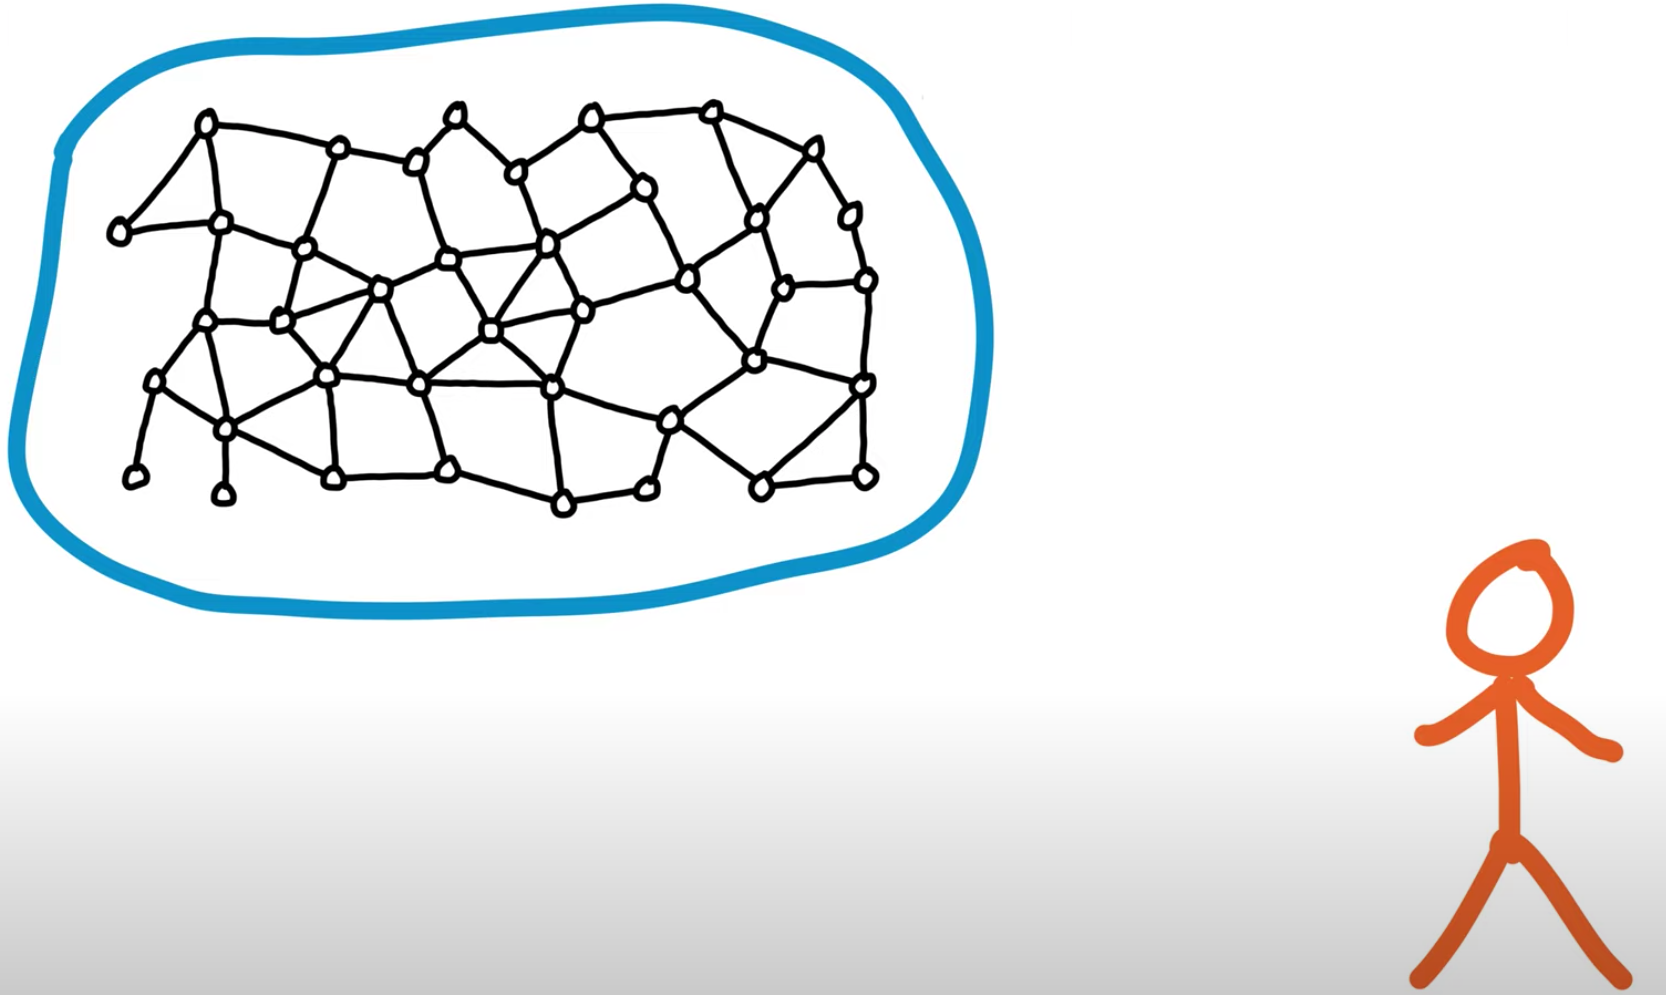
\includegraphics[width=\textwidth]{images/classical-computing.png}
      \caption{Perspective in classical computing}
      \label{fig:classical-computing}
  \end{subfigure}
  \hfill
  \begin{subfigure}[b]{0.49\textwidth}
      \centering
      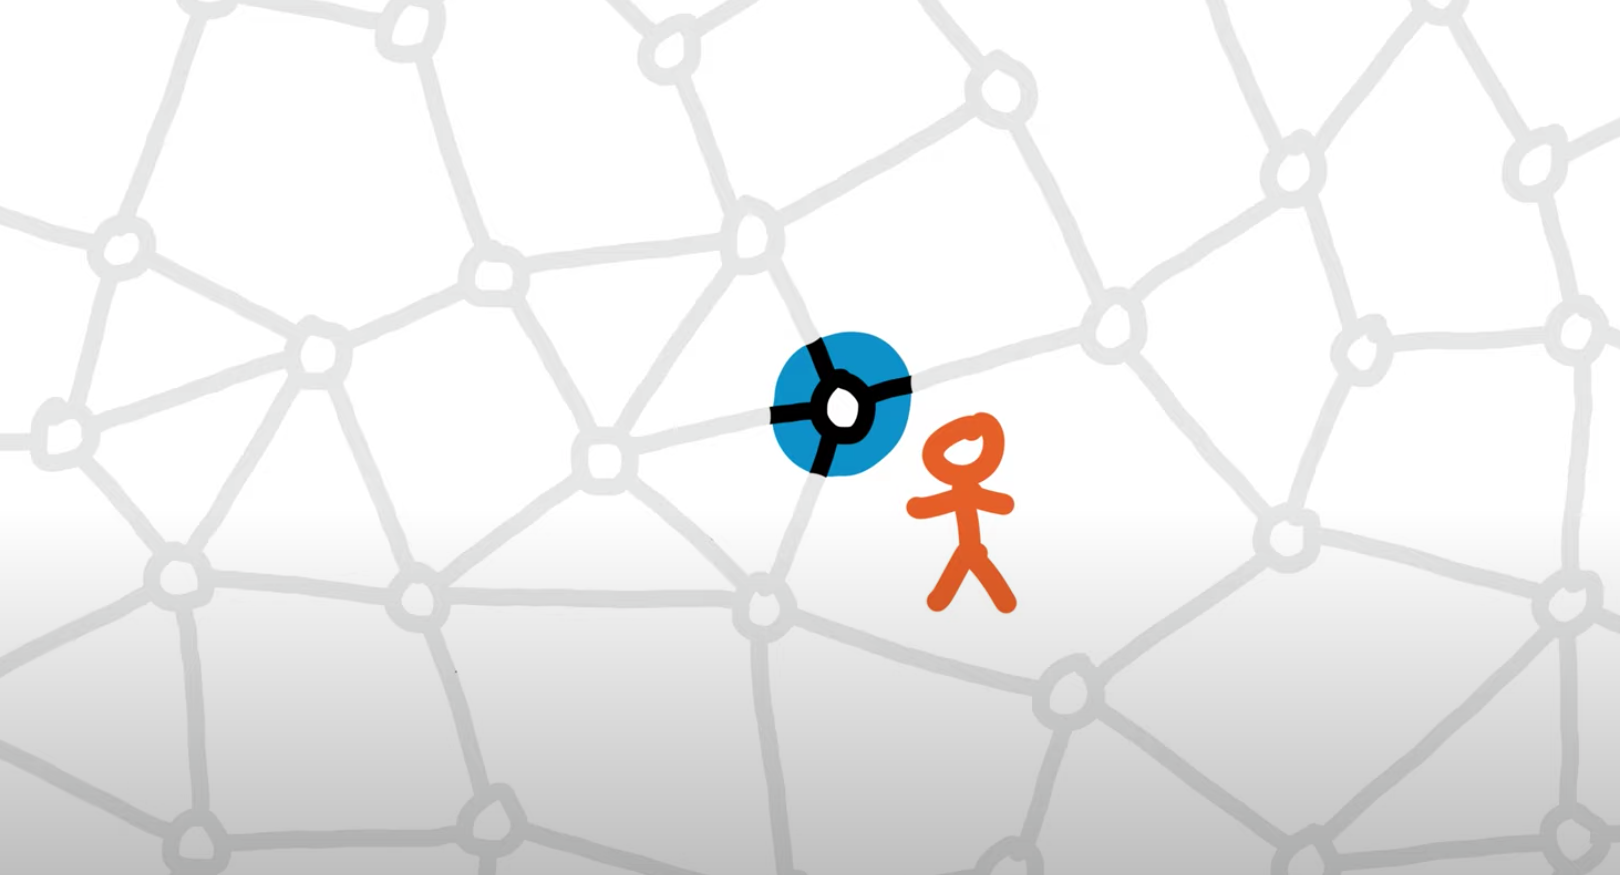
\includegraphics[width=\textwidth]{images/distributed-computing.png}
      \caption{Perspective in distributed computing}
      \label{fig:three sin x}
  \end{subfigure}
  \caption{The difference in perspectives in classical and distributed computing}
  \label{fig:classical-vs-distributed-computing}
\end{figure}

The field of distributed algorithms has several
decades of research history and has grown
in width significantly since its inception in the 1980s.
One specific
area of the field that has received a lot of
attention in recent years from the scientific
community is the study of \emph{locally verifiable}
problems.
These are the kinds of problems, where, roughly speaking,
once execution of an algorithm has ended, each
computational unit can
collect information only from close-by computational units,
and it will be sufficient to ensure that the executed algorithm has succeeded. Problems of this kind are particularly
interesting because they have obvious relevance
in cases where the size of the network is extremely
large, and thus each computational unit
cannot afford to check every other unit in the system.

As the field has been studied, more and more knowledge
about such problems has been accumulated by the
research community. In particular, as is common
in the field of algorithm design, much of the
research has been focused on the complexity of
problems in distributed computing. Apart from
individual complexity results, the research
community has invented several \emph{meta-algorithms}.
These are centralized algorithms that
automatically determine the
computational complexity of a provided
problem.

\section{Problem statement}

The individual complexity results and the meta-algorithms
that determine the complexity of a specified problem are
scattered across tens of published papers. Each of the
papers uses a different problem representation and
formalism. This causes researchers to solve
the same problems again and again since no
centralized place exists that would accumulate all of the
above-mentioned results.

I will attempt to rectify the
situation by designing and implementing a system
that would allow researchers to quickly
access complexity-related results for locally
verifiable problems, provided such problems have been
already studied
previously. I expect that such a solution
would be of high value to the research community and
would save significant time resources, allowing the researchers
to concentrate on discovering new knowledge about the
field instead of spending time on solving problems that
have already been solved numerous times before.

\section{Structure of the thesis}
\label{section:structure} 

Chapter~\ref{chapter:background} provides a theoretical
background necessary for understanding the contents of the
following chapters. The chapter opens with
a brief but informative overview of graph-theoretic
concepts. Then, the chapter provides basic
theoretical background related to distributed computing.
Moreover, the chapter explains notions of
locally checkable problems, decidability, as well as
covers recent developments in the area of
automatic classification in distributed algorithms.

Chapter~\ref{chapter:environment} describes
meta-algorithms that are used in my final
solution. The meta-algorithms take a description
of a locally verifiable problem as an input and
as an output produce some information about the
problem's complexity.

Chapter~\ref{chapter:methods} states my research goals
and defines the scope of the thesis project.
Chapter~\ref{chapter:implementation}
provides an overview of an implementation of
my solution. Chapter~\ref{chapter:evaluation}
evaluates the outcomes of the implementation
against the earlier stated research goals. It
also points out possible directions for
future development. Finally, Chapter~\ref{chapter:conclusions}
summarizes the entirety of the work.


\chapter{Theoretical background}
\label{chapter:background}

In this chapter, we introduce the necessary theoretical background as well as
explain the reasons why the current work is relevant given the latest
developments in the theory of distributed computing. Unless specified otherwise,
the material presented in this chapter is based on the textbook on distributed algorithms by Hirvonen et al.~\cite{Hirvonen2020}.

\section{Graphs}

This section will outline the necessary theoretical background on graphs. 
Most of the notation related graph theoretic concepts in the current
section and in the rest of the thesis will follow that of
a recent introductory textbook on distributed algorithms~\cite{Hirvonen2020},
unless specified otherwise.

A \emph{graph} is a pair $G = (V, E)$, where $V$ denotes the set of all \emph{vertices}
and $E$ denotes a set of all \emph{edges}. Each edge in $E$ is represented as a set of
2 nodes i.e.\ the nodes the given edge is connecting e.g.\ $e = \{v, u\}$ such that 
$v \in V$ and $u \in V$.

When talking about the \emph{size of a graph}, or \emph{cardinality} of the graph, we refer
to the number of nodes in the graph. Or in other words, the size of a graph $G$
is always $|V|$.

Among other things, edges can be categorised into \emph{directed} and \emph{undirected}.
The latter ones simply connect a pair of nodes in a graph, while the latter
ones also contain extra information about which of the two connected nodes is
a ``source'' and which one is a ``destination''. Informally, such a directed edge
can be visualised as an error that starts in a ``source'' node and ends in a 
``destination'' node.  Similarly, we talk about \emph{undirected graphs} -- that is, graphs
where all edges are undirected, and \emph{directed graphs} -- such graphs where all
edges are directed. Formally, while an undirected edge $e$ is defined as a
set of two nodes $e = \{v, u\}$, a directed edge $e$ is defined as a pair
of two nodes $e = (v, u)$. Recall that in the case of a pair, the order of its
elements does matter, hence, the pair allows us to encode the direction of
the edge. Unless mentioned otherwise, we assume that an edge is directed
from the first element of the pair to the second. Also note that in this
thesis, unless specified explicitly, all graphs are assumed to be undirected.

If two nodes are connected by an edge, we call such nodes \emph{neighbours}. We
also say that such nodes are \emph{adjacent} to each other. Moreover, in an undirected graph
if there are two edges $e_1$ and $e_2$ such that $e_1 \neq e_2$ and $e_1 \cap e_2 \neq \emptyset$
such edges are said to be \emph{adjacent} to each other. Similarly, we can talk about adjacent 
edges in a directed graph. In that case, two edges $e_1$ and $e_2$ are adjacent if
$e_1 \neq e_2$ and either first or second element of the pair $e_1$ contains the same
element as either first or second element of the pair $e_2$.

Besides we often talk about edges and nodes being \emph{incident} to each other.
In an undirected graph, an edge $e$ is incident to a node $v$ if and only if $v \in e$. In this
case, we also say that the node $v$ is incident to the edge $e$. Similarly, in a
directed graph, an edge $e$ is incident to a node $v$ if and only if $v$ is the
first or the second element of the pair $e$. Again, in the case described in the
previous sentence, the node $v$ is said to be incident to the edge $e$.

A \emph{simple graph} is an undirected graph where no two nodes are connected by more
than one edge and no edge starts and ends at the same node. In other words, there are
no multiple edges or self-loops in a simple graph.

A \emph{degree} of a node $v \in V$ in a graph $G = (V, E)$ is the number of all
edges incident to $v$. That is, it is the number of edges such that for an edge
$e$, $v \in e$ if $e$ is an undirected edge, or $v$ is the first or second element of
pair $e$ if $e$ is a directed edge. Moreover, for directed graphs, we often talk
about \emph{indegrees} and \emph{outdegrees}. Indegree of a node $v$ is the number
of edges incident to $v$ directed towards the node, while outdegree of a node $v$ is the 
number of edges incident to $v$ directed outwards from the node. Finally, we are 
often interested in a maximum degree of a graph $G$, that is, the maximum value of
degrees of all nodes belonging to the graph $G$. We denote such maximum degree as
$\Delta$

A \emph{walk} in an undirected graph $G = (V, E)$ is a sequence $w$ of a form
$w = (v_0, e_1, v_1, e_2, ..., e_l, v_l)$,
where $v_i \in V$ and $e_i \in E$, and $e_i = {v_{i-1}, v_i}$ for all $i$. A walk from some
node $v$ to some other node $u$ is then a walk $w$ such that its first element i.e.\ $v_0 = v$
and its last element i.e.\ $v_l = u$. Having defined a walk, we can talk about a \emph{
connected graph}. A connected graph, when talking about undirected
graphs, is a graph $G = (V, E)$ in which for any pair of nodes $v$ and $u$ such that
$v \neq u$ there is a walk from $v$ to $u$.

An \emph{isomorphism} between two graphs $G_1$ and $G_2$ is is a function $f$ such that $f$ is a 
bijection, and $f$ maps a vertex of the graph $G_1$ to a vertex of the graph $G_2$, and 
an edge between some nodes $v$ and $u$ exists in the graph $G_1$ if and only if
an edge between nodes $f(v)$ and $f(u)$ exists in the graph $G_2$. From this,
it is rather easy to see that if an isomorphism exists from $G_1$ to $G_2$, then
also an isomorphism exists from $G_2$ to $G_1$. If there exists an
isomorphism between some two graphs, we say that such graphs are isomorphic
(to each other).

A \emph{radius-x neighbourhood} of a node $v$ in a graph $G = (V, E)$ is a set of
all such nodes $u \in V$ that there exists a walk between $v$ and $u$ and 
the shortest walk from $v$ to $u$ is at most $x$. Note that it is possible that
$v = u$, in which case the shortest walk between $v$ and $u$ is 0.

A diameter of a graph (denoted as $\diam(G)$) is the length of the longest walk
in a list $W$, where $W$ is a list of the shortest walks, i.e.\ the one between each pair of nodes
$v$ and $u$ in a graph $G = (V, E)$ such that $v \in V$ and $u \in V$. If a graph
$G$ is nont connected and therefore there is a pair of nodes $v$ and $u$ that do not
have a walk between them, we say that a diameter of such a graph $G$ is infinity. That
is $\diam(G) = \infty$.

\subsection{Several important graph families}

This subsection will introduce some of the graph families that will be necessary
for understanding the content of the thesis. First, we'll define paths and cycles.
Then, we will briefly introduce trees and explain the difference between rooted
and unrooted trees.

A \emph{path} graph is a sequence of nodes that are joined together by edges and
that have the following properties:

\begin{enumerate}
  \item The whole graph is connected. That is, there is a walk from any node of
  the path to any other node of the path.

  \item The graph consists of at least two nodes.

  \item Exactly two nodes have a degree 1 and all the other nodes have a degree~2.
\end{enumerate}

A \emph{cycle} is a connected graph where each node has a degree 2.

A \emph{tree} is an undirected acyclic connected graph. A \emph{rooted tree}
has a single \emph{root vertex}, and thus some nodes have a \emph{parent} node
(some because e.g.\ a root node never has a parent) and one or more \emph{children}
nodes. For a node $v$, a node $u$ is its parent if and only if $v$ and $u$ are
neighbour nodes and the shortest walk from the root to $u$ is shorter by exactly
1 compared to the shortest walk from the root to $v$. Node $v$ is a child of node
$u$ if and only if $u$ is a parent of node $v$. Finally, in the context of rooted trees,
a node $l$ that has no children is referred to as a \emph{leaf} node.
On the other hand, an \emph{unrooted tree} has no single root, and therefore the notion of parent
or child is not defined. Instead, we talk about neighbours of some node $v$. However, we 
still use the notion of leaves to denote nodes of degree 1.

\subsection{Biregular trees}
\label{subsection:biregular-trees}

A \emph{bipartite} graph $G = (V, E)$ has its vertices partitioned into two
subset $U \subseteq V$ and $W \subseteq V$ so that the partitioning forms
a proper 2-coloring of the node $V$. In other words, in a bipartite graph $G = (V, E)$,
if a node $v \in U$ then all its neighbours belong to $W$, and if a node $v \in W$
then all its neighbours belong to $U$.

A \emph{regular} graph is a graph where each vertex has the same degree.
A \emph{biregular} graph is a graph where each vertex has one of the two
allowed degrees and only them. In this thesis, when we talk about
\emph{($\beta$, $\delta$)-biregular} graph $G$, we always assume that 
$G = (V, E)$ is bipartite such that $V$ is partitioned into two
subsets $U$ and $W$, nodes in these subsets form a proper 2-coloring,
all nodes in $U$ are of degree $\beta$ and all nodes in $W$ are of
degree $\delta$. In particular, when we talk about \emph{($\beta$, $\delta$)-biregular trees},
we mean a bipartite biregular tree where all nodes except for leaves
follow the rules of ($\beta$, $\delta$)-biregular graphs described above,
but leaves themselves are allowed to have degree 1 (otherwise they would not be
called leaves).

It is important to notice the equivalence of ($\delta$, 2)-biregular trees
and $\delta$-regular trees. Indeed, given a $\delta$-regular tree, we can
``turn'' each edge $e = \{v, u\}$ into a node $v_e$ such that the node is
connected to node $v$ and $u$ and only those nodes. On the other hand,
given a ($\delta$, 2)-biregular tree, we can remove every node $v$ of degree
2 and, given that nodes $u$ and $w$ used to be neighbours of $v$ before its
removal from the graph, connect nodes $v$ and $w$ with an edge.

\section{Distributed computing}

Now that we have introduced some of the key graph theoretic concepts, we will
next outline some of the foundations of distributed computing. We will start with
a short historical node about the field of distributed computing. Then, we will
explain some of the aspects of the model of computation we're concerned with. Finally, 
we will give some formal definitions to the model of computation that will be our
major concern throughout the rest of the thesis.

\subsection{General background}

The field of distributed computing studies computation in distributed systems, which
have become ubiquitous in the modern world, being especially prevalent
in the area of technology~\cite{Attiya2004}.
A distributed system consists of a number of relatively independent
computing modules, which usually need to cooperate in order to
fulfill a computational task the system has been given. Usually,
each computing module in such a system only has a part of the whole
input and is required to produce only a part of the whole output.
This is in contrast with a centralised system, in which there 
exists an all-knowing entity taking all of the input, performing all
of the computation and producing the whole of a result as its output.
Due to its modularised and parallel nature, distributed computing
has many applications in communication, computation, the Internet,
but also in biology and sociology~\cite{Wattenhofer2016}.

The field of distributed computing appeared already in late 1980s, with several
prominent papers exploring potentialities of computation performed
by multiple interconnected processing units~\cite{Cole1986, Linial1987, Naor1991}.
The first major step in the field happened in 1987, when Linial formalised
some of the principles of one variant of a distributed system.
This model of computation is currently known as Linial's or the \emph{LOCAL model}~\cite{Linial1987}.

\subsection{Model of computation}

Here, we will describe the model of computation that we are going to
assume throughout the rest of the thesis. Note that there is a number
of different models, which are also widely studied in the research
community.

First, as it was already stated, unlike in the case of centralised
computation, we are concerned with multiple interconnected computing entities
that together form a graph. Each such an entity is referred to as a vertex or
a node in a graph. Connections between the vertices are referred to as edges.
The entities only can transfer information along the edges and in no other way
between each other. Unless specified otherwise, the graphs are assumed to be
simple graphs, and all edges are assumed to be undirected. Moreover,
communication along the edges can simultaneously happen in both direction.

Apart from sending infromation to each other, nodes can also
do local computation based on the local information each node possesses. One thing
to note that differs significantly from some of the centralised models of computation
is that each vertex in a graph has arbitrarily huge, but finite, storage and computation resources.
Informally, this means that anything that can be computed in a centralised setting
in a finite amount of time,
can also be computed locally by a node in an arbitrarily small amount of time.
It is also worth noticing that in the model of computation described here,
every node of a graph executed the same algorithm. Nevertheless, the
algorithm might lead to different commands being executed by different nodes
if, for example, nodes' unique identifiers or initial local inputs are different.
Besides, behaviour might also differ if two nodes have somewhat different neighbourhoods
around themselves and therefore will receive potentially different
information during their communication rounds. Finally, at the beginning of
execution, each node knows only its own input (including its own unique identifier
if such has been provided as part of the input) and its own degree i.e.\ the number of
its neighbour nodes in the graph.

Furthermore, computation in a graph happens in synchronous rounds. That implies,
for example, that round $x+1$ is not started by any of the nodes before all of the
nodes have completed round $x$. Moreover, each round is divided into three stages:

\begin{enumerate}
\item Sending some information to some (or all) of its neighbours

\item Receiving information
from some (or all) of its neighbours

\item Performing some local computaiton based
on the information that has been stored by a node locally before and the information
received during the current round from its neighbours

\item Updating its local state i.e.\ replacing and adding data in its own local storage
\end{enumerate}

Each of these stages is also executed
completely synchronously by all nodes in a graph, meaning that e.g.\ no node starts processing
any of its data, before all other nodes have received data from their neighbours. The computation
of a graph is said to be finished when all of the nodes have outputted their final states
and halted. More formally, this means that there are a set of node states that are
considered as ``halting states''. Whenever a node switches its internal state to one of the 
halting state, it does not perform any of the actions from that point in time, or -- to
be even more formal -- it does not send any messages to its neighbours, ignores all of the 
messages sent to it and does not update its internal state in all of the subsequent rounds.
Similar to the requirement that local computation of each node on each round has to be finite
and needs to stop after a finite amount of time passed, all nodes are required to eventually
transition into one of the halting states. That is, a valid distributed algorithm -- in our model of
computing -- cannot continue for an infinite number of rounds. Finally,
the complexity of a distributed algorithm is measured as number of such synchronous rounds
of computation before the algorithm ends i.e.\ before all nodes transition into one of 
the halting states. Notice that different from a centralised model of computation,
algorithms complexity (or in other words its running time) is not affected by the
amount of local computation on a single node.

Another important thing that has to be mentioned when describing the mode of computation
is that all of the operations withing each individual node as well as inter-vertex
communication is absolutely error-free. In other words, all nodes can be assumed to
always act in a fault-free manner, all sent messages can be assumed to never be lost
or undelivered. Therefore, we can always assume that messages sent and received by nodes
are all in accordence to the actual algorithm that is being executed by the nodes 
and not a result of an accidental fault or an intentional adversary effort

\subsection{Distinctive qualities of the LOCAL model}

As was already mentioned previously, our model of computation is known
as Linial's or the LOCAL model~\cite{Linial1987}. Therefore, to complete the
description, we will describe in more detail two distinctive qualities of the LOCAL model
from other models of distributed computing, namely unique identifiers and arbitrarily large
bandwidth.

Each node in the LOCAL model is provided with a unique identifier as part of initial input.
The identifiers are usually assumed to be integer numbers between 1 and $|V|^c$, where
$|V|$ is the number of nodes in the graph and $c$ is some constant. Unless specified, we
assume that such a constant $c$ is not known by the nodes at the beginning of
algorithm execution. Thus, unique identifiers are guaranteed to be positive integer
numbers bounded by a polynomial in the number of nodes, but it is not known -- by the nodes
at the start of algorith execution -- what is the largest unique identifier in the graph. Moreover,
the identifiers of the node do not necessarily form a continuous range of integers. That is,
if an integer $x$ is used as a unique identifier for some node $v$, it is possible
that an integer $x+1$ is not used as an identifier in the graph. This implies that at
the beginning, nodes do not known what integers have been used for unique identifiers
and what have not been, with the exception of only one integer -- their own identifier.

Another characteristic of the LOCAL model, which also was already mentioned before, is the fact
that nodes can send (and receive) an arbitrarily large (but nevertheless finite)
amount of bytes of information over a single edge during one round. This fact,
combined with the existence of unique identifiers, renders the model as a rather strong one.
In particular, this implies that a node can send all of its information -- no matter how
large it is -- to all its neighbours in just one round.

This, in turn, implies a rather
curious property. Imagine that every node sends all of its information during the first round,
and having received some data from its neighbours, saves all this information locally. Consider
some node $v$ in the middle of a graph $G = (V, E)$. Since all nodes send all its data,
after the first round, node $v$
will have all the data that all its neighbours had initially, plus its own initial information.
Notice that each of $v$'s neighbours now have all the information of their neighbours. Thus,
if we combine all the data in posession of $v$ and $v$'s neighbours after the first round, it
is easy to observe that they together have all the information of $v$'s radius-2 neighbourhood.
But this means that after the second round, when all $v$'s neighbours have sent all their
information to $v$, the node $v$ alone posessses all the data that its radius-2 neighbourhood had at the
beginning of the algorithm execution. Similarly, after the 3rd round, $v$ will have all the
radius-3 neighbourhood's data, and so on.
In general, after round $x$, node $v$ will have
all information that was initailly available in its radius-$x$ neighbourhood.
Therefore, when considering the LOCAL model,
time and space are in certain sense equivalent. In other words, the number of rounds
needed to solve a certain problem is always equal to the distance (or radius) to which a node needs to
see to solve a certain problem. One technicality to note here is that because all nodes have
unique identifiers, and these identifiers are sent together with the rest of data,
receiving nodes can differentiate what nodes the received data belongs to, and consequently,
reconstruct the structure of the neighbourhood in the graph.

As a consequence of the above,
we can observe that after $\diam(G)$ rounds, node $v$ will have all the information there is in the 
graph $G$. This implies that after $\diam(G)$ rounds, in the LOCAL model, we can solve anything that can
be solved in a centralised setting. That is, because at the end of $\diam(G)$'th round, each node in the
graph have collected all the information there is in the graph and thus can just run the
computation locally. And because local computation in the LOCAL model is virtually free,
anytihng that could be computed in a centralised setting will be computed locally by each
node individually. On the next round, each node can output their part of the solution.

\subsection{Formalising the LOCAL model}

In this subsection we will formalise LOCAL model that we informally described above.
This will, first of all, help to clarify the aspects of the model that are still left ambiguous
after reading the previous subsections. Besides, it will allow us to introduce
a randomised model below once the basic deterministic one is unambiguously defined.

An algorithm being executed by each node consists of 
three functions. One for local state initialization that is executed only once, after
a node $v$ has received its initial local inputs $u(v)$ but before the first round
$$\init_A(u(v), d)$$
where $A$ is a given distributed algorithm and $d$ is the degree of the node $v$.
The function return an initial local state of the node $v$.

The second function takes as an input an internal state $x(v)$ of a node $v$
and returns a tuple of size $d$, where $d$ is a degree of node $v$. The
tuple contains messages that are to be sent to $d$ neighbours of the node $v$
during the current round.
$$\send_A(x(v), d)$$
The third function takes as an input a local internal state $x(v)$ of a node
$v$, and a tuple $m(v)$ of size $d$ that contains messages received from $d$ neighbours
of the node $v$.
$$\receive_A(x(v), m(v), d)$$
The function returns a new local internal state of the node $v$, which becomes a
starting internal state $x(v)$ in the next round.

\subsection{Randomised algorithms}

This subsection will introduce a randomised distributed model of computation
and highlight some of the difference between randomised and deterministic
models. In this section, the focus will be specifically on the randomised LOCAL
model as opposed to some other distributed algorithms models.

In the randomised LOCAL model, we have two major differences from the
deterministic LOCAL model. First, the function $init_A(u(v), d)$ becomes
randomised. This means that the initial state $x_0(v) = init_A(u(v), d)$ of a node $v$ is
chosen from a discrete probability distribution of all possible initial states.
Second, the function $receive_A(x(v), m(v), d)$ becomes randomised. This means that,
after all messages have been sent and received for round $i$, a new local internal
state $x_i(v) = receive_A(x(v), m(v), d)$ for a node $v$ is selected from a
discrete probability distribution. Everything else in the model remains exactly
as it is in the deterministic case, that is, no changes are made to the $send_A(x(v), d)$
function.

Since probabilities are involved when in randomised setting, it might not be
drectly obvious what it means to ``solve'' a problem. The major problem is that
since states of the nodes are chosen from a discrete probability distribution,
there is always a probability that the output of the nodes will not be valid.
Therefore, there is often a probability that the problem has not been solved
after a certain number of rounds.

But before we define what it means to solve a problem in a randomised setting, it's
worth noting that there exist two kinds of randomised algorithms: ``Monte Carlo'' and
``Las Vegas''. \emph{Monte Carlo} algorithms always stop after a specified $f(n)$
number of rounds, where $n$ is the number of nodes in the graph, but
it is not guaranteed that the output will a valid one. Monte Carlo algorithm
only guarantee their execution time, and succeed only with probability $p$.
\emph{Las Vegas} algorithms, on the other hand, always produce a correct output,
once all the nodes in a graph have stopped, but the algorithm will stop after a
specified $f(n)$ number of rounds only with some probability $p$. Thus, in some
way, these types of randomised algorithms are complements of each other:
one guarantees correctness of the output but has a chance of going over some
specified execution time, while another has a guarantee on the execution time
but has some probability of producing incorrect output. In the rest of the thesis,
unless explicitely specified otherwise, we assume that the randomised algorithms
are Monte Carlo algorithms.

Finally, we now can define what it means to solve a problem in a randomised context.
When saying that a certain randomised algorithm ``solves'' a cerrtain problem in
$T(n)$ rounds, unless specified otherwise, we mean that the algorithm stops after
$T(n)$ computational rounds and the nodes output (or to be more precise the nodes
have transitioned to one of the output states) a correct solution ``with high
probability'' (often denoted as ``w.h.p.''). Formally, if an algorithm succeeds with
high probability, it means that the algorithm succeds with probability of at least
$1 - 1 / n^c$, where $n$ is a number of nodes in a graph and $c$ is some constant
such that $c > 0$. Moreover, $c$ is a constant that can be freely chosen when 
running the algorithm. To give a simple example, an algorithm's running time may
linearly depend on such a constant $c$, then before an algorithm is executed,
one may freely choose the constant so that the larger the constant the longer is
the running time, but also the lower the chance that the produced output will
be incorrect. Notice that $c$ does not need to affect running time, but it often
does since the larger it is the lower is the probability of algorithm's failure,
and decreasing such probability usually comes at the cost of something else -- 
often running time. Thus, when saying that something succeeds ``with high probability''
we do not mean it vaguely but rather refer to a very precise mathematical definition
given above.

\section{Iterated logarithm}

This section will introduce the iterated logarithm function. The function is
one of the most common complexity results of distributed algorithms and will
appear often in the rest of the document.

The interated logarithm function, denoted as $log^*(x)$ is defined as follows:
\[
    \log^*(x) = \begin{cases}
        0 & \text{ if $x \le 1$}, \\
        1 + \log^*(\log_2 x) & \text{ otherwise}.
    \end{cases}
\]
The function is notable for the fact that it grows extremely slow. For example,
\begin{align*}
  &\log^*(1) = 0, \\
  &\log^*(2) = 1, \\
  &\log^*(4) = 2, \\
  &\log^*(16) = 3, \\
  &\log^*(65536) = 4, \\
  &\log^*(2^{65536}) = 5.
\end{align*}

\section{Locally Checkable Labelling problems}

This section will introduce locally checkable labelling problems (from now on referred to as
LCLs), which are the main focus of this thesis. The section will start with
a short historical note and then provide a formal definition of
LCL problems.

As the field of distributed algorithms started to develop, it became clear
that some classes of problems
are of a particular interest to the theoretical research community.
One class of such problems has been first introduced in 1993 by
Moni Naor and Larry Stockmeyer under the name of Locally Checkable 
Labelling (LCL) problems~\cite{Naor1993}.

In short, an LCL problem is a distributed problem that satisfies the 
following criteria~\cite{Naor1993, Suomela2020}.

\begin{itemize}

\item the maximum degree of a graph is a finite number that does not depend on $n$,

\item there is a finite number of input labels and the number is not dependent on $n$,

\item there is a finite number of output labels and the number does not depend on $n$,

\item the correctness of a solution can be checked locally by each individual node. That is,
after a solution is produced and all the nodes in the graph have stopped, each node can just
check a radius-$O(1)$ neighbourhood around itself. The solution is valid if and only if each of
the individual neighbourhoods for all the nodes are valid.

\end{itemize}
In the list above, $n$ is the number of nodes in the graph. Finnally, as is easy to see from the definition of LCL
probles
above, there is always a finite representation of any LCL problem. Indeed, one can simply list
all valid local neighbourhoods, list all valid input labels, list all valid output
labels and specify the maximum degree of a graph. Since all of the beforementioned are
of size $O(1)$, it is always possible to have a finite representaion of an LCL.
In practive however, it is in many cases more practical to come up with
a more concise representation. We will return to the topic of representing LCL
problems later in this thesis.

The study of LCL problems has been one of the major research directions
during the last 6--7 years, with numerous papers published in major
distributed computing conferences
~\cite{Balliu2016, Chang2016, Brandt2017, Chang2017, Fischer2017a, Rozhon2019, Balliu2020-1, Balliu2020-2}.
Currently, the study of LCL problems has reached the stage of maturity with,
for example, the complexity landscape of LCL problems understood
almost entirely ~\cite{Suomela2020, Chang2020a}.

\section{Major LCL problems}

This section will introduce some of the common LCL problems
widely studied in distributed algorithms research community.
Note that all of the problems also exist in the context of 
centralised computing.

\textbf{Vertex coloring} is perhaps one of the most well-known
problems on graphs. Informally, the goal is to color a graph
in such a way that no two adjacent nodes are colored with the
same colors. It is also easy to see tshat the problem is an
LCL problem because it is sufficient and necessary for each node to check
its radius-1 neighbourhood. If each node's radius-1 neighbourhood is
a valid one i.e.\ none of the neighbours of node $v$ have the same color as $v$
itself, then and only then the output is a valid vertex colorings

Another well-known and widely studied problem on graphs is
\textbf{edge coloring}. Informally, each edge needs to be
colored in such a way that no two adjacent edges are of the same
color. Coloring edges in a graph can still be simulated
with the setting in which only nodes output the labels.
Each node will output a tuple of the size equal to the node's
degree. Each element of a tuple represents a label
that the node outputs on a coresponding edge. The problem
is also an LCL problem, because after a final output is
produced, each node $v$ will need to check its radius-1
neighbourhood to make sure two things are in order:
\begin{enumerate}
  \item All edges incident to $v$ have to be of different color.
That is, no two elements of node $v$'s output tuple should be the same.

  \item For each edge incident to $v$, a color that node $v$ colored some incident
edge $e$, should be the same as the color that node $u$ colored the edge $e$ with.
Here $e = \{v, u\}$. In other words, because each edge's coloring depends on
output of two nodes, such coloring has to be consistent for each edge i.e.\ the produced
colors need to be the same on both ends of each edge.
\end{enumerate}

An \textbf{independent set} is a set $I$ of vertices in a graph $G = (V, E)$ such that
$I \subseteq V$. The only condition, however, is that no pair of vertices in the set $I$
can be adjacent to each other. A \textbf{maximal independent set problem} is then a
problem in which in addition to finding such independent set $I$, there is an additional
maximality restriction. The maximality restriction forbids cases where a node $v$
is not in the set $I$ but also does not have any adjacent nodes in the set $I$.
In other words, in a \textbf{maximal independent set} all nodes either belong
to the set $I$ or they \emph{cannot} join it because one of their neighbours has
already joined. It is trivial to see that the problem is an LCL as checking local
eighbourhood will suffice to determine if the solution is valid or not.

\begin{figure}
  \centering
  \begin{subfigure}[b]{0.49\textwidth}
      \centering
      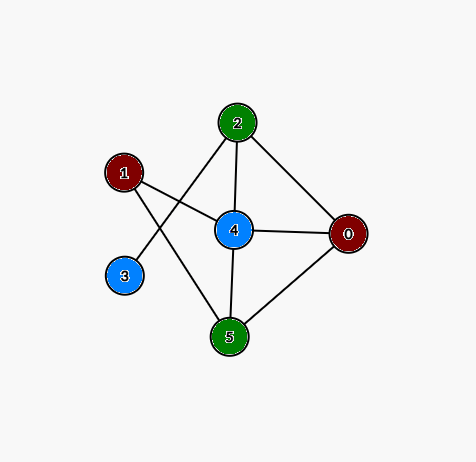
\includegraphics[width=\textwidth]{images/vertex-coloring.png}
      \caption{Vertex coloring}
      \label{fig:vertex-coloring}
  \end{subfigure}
  \hfill
  \begin{subfigure}[b]{0.49\textwidth}
      \centering
      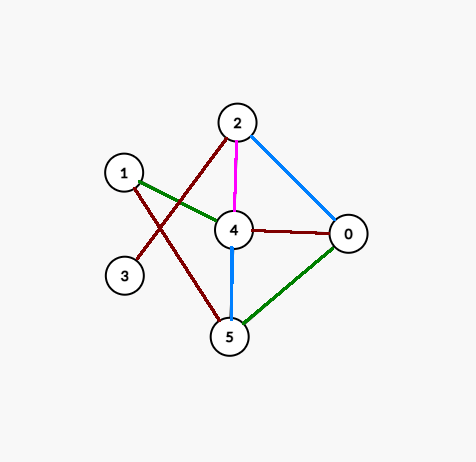
\includegraphics[width=\textwidth]{images/edge-coloring.png}
      \caption{Edge coloring}
      \label{fig:edge-coloring}
  \end{subfigure}

  \hfill
  \begin{subfigure}[b]{0.49\textwidth}
      \centering
      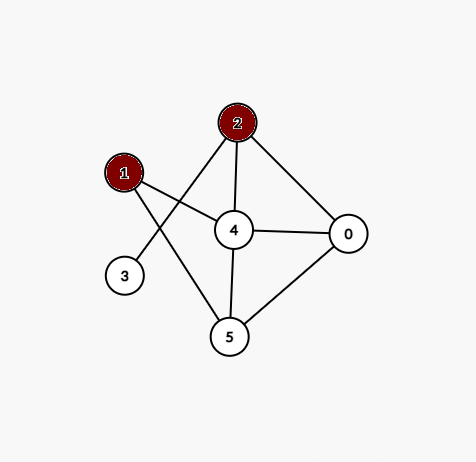
\includegraphics[width=\textwidth]{images/maximal-ind-set.png}
      \caption{Maximal independent set}
      \label{fig:maximal-independent-set}
  \end{subfigure}
  \hfill
  \begin{subfigure}[b]{0.49\textwidth}
      \centering
      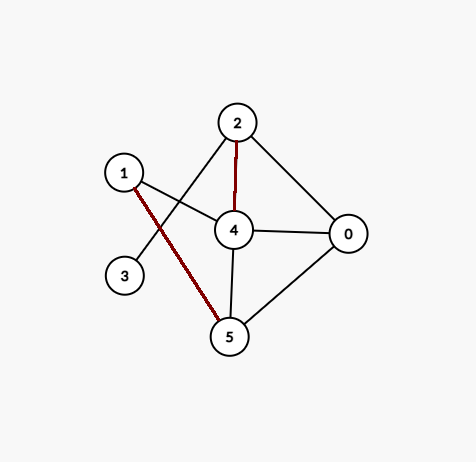
\includegraphics[width=\textwidth]{images/maximal-matching.png}
      \caption{Maximal matching}
      \label{fig:maximal-matching}
  \end{subfigure}
  \caption{Some of the common LCL problems}
  \label{fig:graph-problems}
\end{figure}

Finally, a \textbf{maximal matching problem} is a problem in which nodes need to
produce a matching such that each node is either matched with one of 
its neighbours or it cannot be matched because all of its neighbours are
matched. That is, no node can be left unmatched while at least one of its
neighbours is unmatched. It is trivial to see that the problem is an LCL
since each node can check its radius-1 neighbourhood to check whether it
is matched with a neighbour or all neighbours are matched with someone else.
And if the condition of the previous sentence is not satisfied, the output
is invalid.

\section{Decidability and undecidability}

Before moving forward, it is important to remind about a notion of
decidability in the context of theoretical computer science. It is
assumed that the reader already has some basic knowledge on
complexity theory, computability, Turing machines, automata and
languages. The content of this section follows
definitions and formalisms as defined in of Sipser~\cite{Sipser2012}
unless specified otherwise.

First of all, recall that a deterministic Turing machine is called
\emph{decider} if it halts on all inputs. Similarly,
a nondeterministic Turing machine is called a decider, if
it ends up in a halting state in all of its branches. We then
call a language \emph{decidable} if and only if there is some Turing
machine that decides it. That is, a language $L$ is decidable
if and only if there exists some Turing machine $M$ that given
and input $x$, such that $x \in L$, always halts.

\emph{A decision problem} is an algorithmic problem, that has only two
valid solutions to it: ``yes'' and ``no''. We assume that a decision
problem has an infinite set of inputs. That is, a decision problem
defines an infinite but possible restricted set of valid inputs,
and for each input only one of the two outputs is the correct
output. An algorithm is said to solve a problem $P$ if and only
if, given any input from a set of valid inputs, it can
always produce the correct output. Recall also that we can
represent any decision problem $P$ as a formal language $L_P$, where
a string $x \in L_P$ if and only if, given that $x$ is an input
to the problem $P$, the correct output is ``yes''. To clarify,
for each problem $P$, there is a language $L_P$ such that
if $P$'s output on some input $x$ is ``yes'', then $x \in L_P$,
otherwise $x \notin L_P$. From now on, we will call such
language $L_P$ that ``represents'' a decision problem $P_L$ as
\emph{corresponding language} of problem $P$.

Then, a decision problem $P$ is \emph{decidable}, if and only if
there is a decidable corresponding language $L_P$.
On the other hand, a decision problem is \emph{undecidable},
if and only if, there is no decidable corresponding language $L_P$.
Note that a problem is undecidable if and only if it is not
decidable.

To prove that a problem $P$ is decidable, it is sufficient to
show an algorithm (formally a Turing machine) $A$, such that
$A$ correctly solves the problem for all valid inputs. That is,
such an algorithm $A$ must always halt and must produce the
output ``yes'' if and only if it is the correct output of the
problem $P$ given the input. Thus, proving decidability
requires finding such an algorithm, and then proving
that $A$ always halts and that $A$ is indeed correct.
To prove that a problem is undecidable is however less
trivial. One of the common techniques is to show that
the problem can be reduced to the Halting problem~\cite{Margenstern2000, Turing1937}.

\section{Automatic synthesis and classification}

\emph{Automatic classification}, broadly speaking, is a problem
where objects of certain type that possible share some
properties in common are required to be classified into
several, often in-advance known categories automatically,
that is, without or with minimal human supervision.
Due to the recent successes in the field of machine learning,
numerous automatic classification problems have been solved,
or at least for many of the problems, significant
progress have been made. In particular, automated classification
of image, sound and text data
based on deep neural networks -- one of the popular machine learning
techniques that have had multiple breakthroughs in the recent years --
had some significant results in the areas of medicine, biology,
agriculture and many others~\cite{auto-class_Sharma2017,
auto-class_Capizzi2015, auto-class_Ibrahim2018, auto-class_Colonna2016,
auto-class_Winkler2017, auto-class_FabioDelFrate}.

However, automatic classification is also possible beyond
the physical media such as images, sounds, etc. For example,
it is often useful to classify abstract problems, e.g.\ mathematical
or computer science problems. Indeed,
Fulton et al.~\cite{class_Fulton} have shown an approach
for automatic classification of Sturm-Liouville
problems~\cite{zettl2010sturm}.

\emph{Automatic synthesis} is a problem of automatically
synthesizing or finding
a solution to a certain problem given a set of constraints and/or
objectives. For example, automatic synthesis is fairly common
in the field of electrical engineering, and is commonly
applied when designing analog and digital circuits~\cite{synthesis_,
synthesis_autoAx}. Furthermore, with the recent rise in popularity
of quantum computing, the need has arisen for design of quantum
circuits. Similar to the classical cases, synthesis of
quantum circuits have become a popular research direction
with numerous publications on the matter~\cite{synthesis_Khan2017,
synthesis_Meuli2018, synthesis_Miller2003}.

In general, algorithm synthesis in the context of theoretical
computer science is undecidable. However, there are some
research directions in the field of distributed computing and
distributed algorithms, where some forms of automatic synthesis and/or
automatic problem classifications have led to succesfull
developments~\cite{Balliu2018, da-synthesis_Rybicki2015,
da-synthesis_Klinkhamer2016,
da-synthesis_Hirvonen2017, da-synthesis_Fathiyeh2015, da-synthesis_Dolev2016,
Chang2017, Brandt2017, da-synthesis_Bloem2016}. Moreover,
the notions of automatic synthesis and automatic classification are
often interconnected in the context of distributed algorithms.
To demonstrate this, we take an example of a common problem in
a distributed computing: given a problem $\Pi$, we need to
automatically determine its compelxity. Assigning a complexity
class to the problem $\Pi$ can be viewed as classification
problem here. On the other hand, proofs of the type that
demonstrate that $\Pi$ belongs to a certain complexity class
are often constructive in nature. That is, to show that a
problem can be solved in the number of rounds $x$, we
often need to develop and algorithm that solves the problem
in the stated number of rounds. But developing such algorithm
can potentially be automated, meaning that \emph{automatic
algorithm synthesis} can be used. Thus, in the context of
distributed computing, automatic algorithm
synthesis and automatic problem classification are often two perspectives
on the same thing: determinging whether a problem $\Pi$ can be solved
in $x$ rounds or is it fundamentally more difficult.

\section{Recent developments in automatic classification of LCL probems}

At this point that the theoretical background has been given, it is
useful to give a background to much more recent developments in the
distributed algorithms research. As the branch of research of
studying LCL problems had been reaching maturity, many focused
on the idea of automated classification of LCL problems. That is,
the question of interest is whether we can create meta-algorithms
that would take the description of an LCL problem as its input
and produce the problem's round complexity as an output.
This being the core topic of the thesis, it is thus important
to describe all the prior work done in this direction.
In the rest of the
section, we will introduce some of the negative as well as positive results
related to automated classification of LCL problems.

The questions of whether a certain class of LCL problems
can be automatically classified are often referred to
as decidability questions. Roughly speaking, a problem is
said to be decidable if there exists an algorithm that,
given the problem, will output its complexity. Such decidability
questions are often studied in relation to the whole
family of graph problems and not to individual instances
of problems.

\begin{figure}[ht]
  \begin{center}
    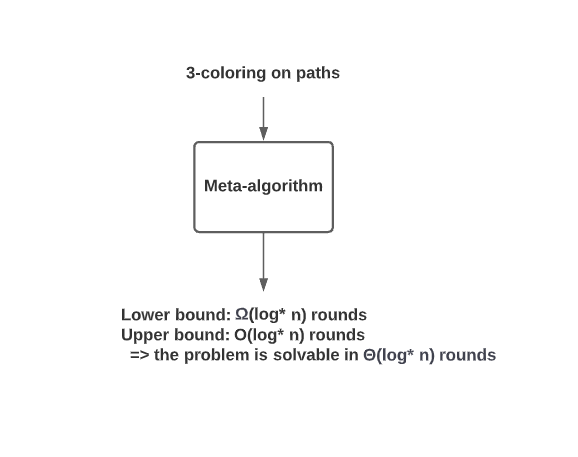
\includegraphics[width=\textwidth]{images/meta-algorithm.png}
    \caption{Conceptual representation of a meta-algorithm}
    \label{fig:meta-algorithm}
  \end{center}
\end{figure}

First of all, it is important to notice that it has been
proven that in general LCL problems are undecidable.
In fact, already in the cases when the graph family is a grid,
LCL problems cannot be automatically classified~\cite{Brandt2017, Naor1993}.

Nevertheless, many interesting LCL problems are still decidable.
For example, it was known for several years now that LCLs
on paths and cycles are decidable~\cite{Balliu2018, Brandt2017, Naor1993}.
Besides, certain types of LCL problems are also decidable on
trees~\cite{Chang2017}.

But the fact the a problem is decidable in theory does not
always imply that it is possible in practice to
construct an algorith for automatic classification of
such problems. For instance, it is known that even in
the case of paths and cycles, if a node labelling is
given as part of the input, decidability becomes
PSPACE hard~\cite{Balliu2018}.

However, not everything looks that gloomy, and many
interesting and sufficiently broad families of LCL
problems are both decidable and possible to
automatically classify in practice. Indeed a lot of work
has been done attempting to derive practival algorithms
that determine complexity of a given LCL problem,
especially in trees.

Balliu at al.~\cite{Balliu2019c} has shown that a complete classification
of binary labelling problems (problems where a node's
output is allowed to be only one of the two possible labels)
at least in a deterministic setting is possible and moreover
can be done in $O(1)$ time, since computational
complexity of such problems can be simply looked up in a
table in a constant time. In addition
to this, the paper also shows that it is decidable to
classify at least \emph{some} of the randomised binary labelling
LCL problem~\cite{Balliu2019c}.

Building on top of the work outlined in the paper, Rocher~\cite{Rocher2020clas}
has developed a meta-algorithm that classifies \emph{almost}
all ternary labelling problems on trees in deterministic
setting. Furthermore,
he also implemented the meta-algorithm as a
computer program written in Python programming language~\cite{Rocher2020doc}.
Although the implementation focuses mainly on the case of trees with degree 3,
the techniques described in the manuscript are applicable to ternary problems
on trees of higher degrees as well.

In addition to this, LCL problems on trees and cycles
are fully decidable in polynomial time as was shown by Chang et al.~\cite{Chang2020}.
The algorithm for classifying the problems can be used in practice and has
been implemented in Python programming language by Aalto's
Distributed Algorithms research group~\cite{Tereshchenko2020}.

Furthermore, a technique called round elimination was introduced in the context
of LCL problems by Brandt et al.~\cite{Brandt2019}. It is a series of mechanical
steps that, if followed, in many cases transform an LCL problem $\Pi_0$ into another LCL problem $\Pi_1$. An interesting property is that, given certain assumption and the fact that
$\Pi_0$ is solvable in constant time e.g.\ in $T$ rounds, $\Pi_1$ is guaranteed to be
solvable in exactly $T - 1$ rounds. This single property has numerous implications.
For example, if we apply the technique $k$ times and in the end obtain an LCL problem $\Pi_k$
such that it is zero-round solvable, we know that the original problem $\Pi_0$ is
exactly $k$-round solvable. Moreover, round elimination is not only possible
in theory but is also very much feasible in practive.
Indeed, Olivetti~\cite{Olivetti2020} has
implemented a computer program that, given an LCL $\Pi_0$ solvable in $T$ rounds,
it produces another LCL $\Pi_1$ solvable in $T - 1$ rounds. There even exists
a web interface for the program, and one can apply the technique and obtain
its results within milliseconds. We will describe the technique and its implications
in much more detail in the subsequent section.

Finally, very recently, Balliu et al.~\cite{Balliu2021} demonstrated
that LCL problems on rooted trees are completely decidable.
In particular, an LCL problem on rooted trees can be completely
classified in both deterministic and randomised settings. The only
exception to this completeness is deciding whether a given problem
has round complexity of $\Theta(n)$ or it is unsolvable. In addition
to the theoretical results in he manuscript, the authors also
provide a freely available open souce software that is able to
classify an LCL with relatively small number of labels in a matter
of milliseconds~\cite{Studeny2021}.


\chapter{Meta-algorithms used in the solution}
\label{chapter:environment}

This chapter will describe in detail all the meta-algorithms that are
used in the final solution as subroutines.
Chapter~\ref{chapter:implementation} will then
describe how the final solution was built on top of the meta-algorithms
described in this chapter.

\section{Round elimination}

This section explains in detail round elimination (RE)
technique introduced in Chapter~\ref{chapter:background}, as well as
implementation of round elimination technique as a computer
program written in Rust \cite{Brandt2019, Olivetti2020}.
Besides, I will demonstrate that all LCL problems that
we're interested in can be represented in a formalism
of round elimination, which implies
its wide applicability.

As already mentioned in the previous chapter, round elimination
is a technique that, given an LCL problem $\Pi_0$ as an input, produces
another LCL problem $\Pi_1$ which can be solved exactly one round
faster. For round elimination to work, the input must comply
to the following two constraints: $\Pi_0$ has to be a problem on a $(\delta, \beta)$-biregular
graph, and the number of rounds in which $\Pi_0$ can be solved
should not be ``too large''. Indeed, the last constraint is a rather curious one
since we rarely know round-complexity of an input problem when using
round elimination. However, we can nevertheless use this rather inconvinient constraint
to our advantage, which will be demonstrated below.

Furthermore, when applying round elimination, we talk about \emph{active} and
\emph{passive} nodes. Since $(\delta, \beta)$-bipartition of an input problem is
already given (see our assumption above), nodes of degree $\delta$ are assumed
to be active and nodes of degree $\beta$ are assumed to be passive. For a problem
to be a valid input to round elimination, it has to be reformulated as a problem on
a $(\delta, \beta)$-biregular graph where only one partition of nodes produces
some output while the other partition does not produce any output but instead
checks that their radius-1 neighborhood's outputs comply to previously
specified restrictions.

In order to demonstrate the technique, we will have as our running
examples two canonical problems: weak 3-labeling and sinkless orientation.

\textbf{Weak 3-labeling} in this context is a problem on $\delta$-regular trees where
each node labels its incident edges in such a way that no node $v$ in the graph
has all its incident edges labeled with the same label. Besides if two
nodes $v$ and $u$ are incident to the same edge $e = \{v, u\}$, such
edge $e$ has to be labeled with the same label from both ``sides''. In other words,
two neighboring nodes cannot output different labels on the same edge.
It is easy to see that, although the initial problem is specified for a regular
tree, we can obtain an equivalent problem for a $(\delta, 2)$-biregular tree
by replacing edges with nodes as described in Section ~\ref{subsection:biregular-trees}.
Further, if we assume that all nodes of degree $\delta$ are active and all nodes of 
degree 2 are passive and that nodes of degree $\delta$ cannot have their incident
edges labeled all with the same label, and nodes of degree 2 must have both of their
incident edges labeled with the same label, we obtain an LCL problem equivalent to
weak 3-labeling but in a formalism suitable for round elimination. To formalise, we
can define the problem as follows:
\begin{align*}
\Sigma &= \{A, B, C\}, \\
A &= \{ \{A, B, C\}, \{A, A, B \insetor C\}, \{B, B, A \insetor C\}, \{C, C, A \insetor B\} \}, \\
P &= \{ \{A, A\}, \{B, B\}, \{C, C\}\},
\end{align*}
where $\Sigma$ is an allowed alphabet, $A$ is a set of \emph{configurations}
allowed for active nodes, and $P$ is a set of configurations allowed for
passive nodes. Here, we assumed that $\delta = 3$. Notice that each
configuration is a set of labels that are allowed to be outputted on ports
incident to any active/passive node $v$. Notice also that the order of
the labels in a single configuration does not matter. Finally, in this particular problem
and in all problems in the context of round elimination, we usually do not care about
leaf nodes. That is, leaf nodes are unconstrained and are fine with any 
configuration.  Next, I will
describe another problem using the same formalism.

\textbf{Sinkless orientation} (SO) is a problem
where each non-leaf node has outdegree of atleast 1.
We will consider the problem in the context of
a $\delta$-regular tree.
Notice that we can interpret $\delta$-regular
tree as a
$(\delta, \delta)$-biregular tree with
both active and passive nodes being of degree $\delta$.
Recall also that since the tree is biregular, we
necessarily assume bipartition of the nodes. In other words,
we assume that 2-coloring is already given for the tree.
Then, we can define the problem formally as follows:
\begin{align*}
\Sigma &= \{I, O\}, \\
A &= \{ \{O, I \insetor O, I \insetor O\} \}, \\
P &= \{ \{I, I \insetor O, I \insetor O\}\}.
\end{align*}
Here we again assumed that $\delta = 3$. Label $I$ here represents
an incoming edge and label $O$ represents an outgoing edge.
Note that because the labels are produced only by active nodes,
outgoing edge $O$ for an active node is an incoming edge for a 
passive node. And vise versa: an incoming edge $I$ for an active node
is an outgoing edge for a passive node. Thus, the sets of configurations
$A$ and $P$ can be interpreted so that each node -- no matter active or passive --
has to have at least one outgoing edge, and the rest of the edges can be anything.

Now that I have defined our two example problems,
I will apply round elimination
technique on each one, describe intermediate steps, and analyse the results.
Notice that the low-level technicalities of round elimination
are omitted in the current thesis for brevity. For in-depth technical details, a reader is encouraged
to refer to the original paper by Brandt~\cite{Brandt2019} or to the recently published textbook on distributed algorithms
by Hirvonen et al.~\cite{Hirvonen2020}.

Let us denote the initial weak 3-labeling problem as $\Pi_0$. After applying round elimination, we get as its
output another LCL problem $\Pi_1$. The formal description of the problem is as follows:
\begin{align*}
\Sigma &= \{A, B, C\}, \\
A &= \{ \{A, A\}, \{B, B\}, \{C, C\}\}, \\
P &= \{ \{A, B ,C\}, \{A, A, B \insetor C\}, \{B, B, A \insetor C\}, \{C, C, A \insetor B\} \}.
\end{align*}
The problem $\Pi_1$ is not zero round solvable since after zero rounds each node only
knows its own degree and unique identifier. Thus, no matter what is the mapping from
unique identifiers to the output is, we can construct such a graph, where there exists
a passive node whose all three neighbors will output the same label. But set $P$ does not
contain any configurations consisting of the same three labels, therefore such
output would be invalid. So we just have another problem that looks a lot like our
previous problem $\Pi_0$ (essentially sets $A$ and $P$ have simply been swapped).
Let us run round elimination once again, now using $\Pi_1$ as its input. We obtain
$\Pi_2$, which looks as follows:
\begin{align*}
\Sigma &= \{A, B, C, D, E, F, G\}, \\
A &= \{ \{C, E, F\}, \{C, D, G\}, \{B, E, G\}, \{A, F, G\}\}, \\
P &= \{ \{ACEG, ACEG\}, \{BCFG, BCFG\}, \{DEFG, DEFG\} \},
\end{align*}
where we use $X_1X_2...X_k$ notation to mean the same as $X_1 \insetor X_2 \insetor ... \insetor X_k$.
Now this problem is zero round solvable. Indeed, if all active nodes output $\{C, E, F\}$
on their incident edges in an arbitrary order, passive nodes will be satisfied (that is to say
that all passive nodes will find a configuration from the set $P$) in all cases.

Now since we know that $\Pi_2$ is 0-round solvable, using the justification already described
above, we can conclude that our original problem $\Pi_0$ is exactly 2-round solvable. Thus,
weak 3-labeling on $(3, 2)$-biregular graphs is solvable in $O(1)$ rounds. Observe that
we have just used round elimination technique to \emph{prove} that an LCL problem can be
solved in constant number of rounds.

Next, we will analyse SO in a similar manner. Let us again denote SO as $\Pi_0$ and apply
round elimination to it. We obtain the following output problem:
\begin{align*}
\Sigma &= \{A, B\}, \\
A &= \{ \{A, B, B\} \}, \\
P &= \{ \{B, AB, AB\}\}.
\end{align*}
Applying round elimination once again, we get
\begin{align*}
\Sigma &= \{A, B\}, \\
A &= \{ \{A, B, B\} \}, \\
P &= \{ \{B, AB, AB\}\}.
\end{align*}
It turns out that $\Pi_2 = \Pi_1$. But we also know that round complexity of $\Pi_2$
has to be smaller by 1 round than that of $\Pi_1$. Although this sounds like a contradiction,
it turns out that the key here is to pay attention to the initial assumptions that I mentioned at the
beginning of the section. Namely, the number of rounds $T$ of the original problem cannot be ``too large''.
Hence, in the case of SO, the number of rounds necessary to solve it is ``too large''. Moreover,
it has been shown that in cases like this, when, after applying round elimination repeatedly,
we encounter a problem that we have already seen before, the initial problem $\Pi_0$, in most of the cases,
is solvable in $\Omega(\log n)$ rounds in deterministic setting and in $\Omega(\log \log n)$ rounds
if randomness is allowed. Thus, we can use round elimination not only to prove upper bounds but
also lower bounds for LCL problems on biregular graphs.

Although I have only demonstrated the technique for two problems, the same idea following for most of the
other LCLs on biregular graphs. In general RE can be used in an atomatic manner to prove constant upper or
logarithmic and polylogarithmic lower bounds for a wide range of LCL problems. Furthermore, the open-source
implementation
of the technique written in programming language Rust and publicly available as a command-line tool and via
a web interface will hugely assist in using RE as part of my software solution for automated classification
of LCL on trees.

Finally, it is worth demonstrating that the formalism used in round
elimination (and in the Round Eliminator implementation) is universal.

\begin{theorem}\label{theorem:re_formalism_is_general}
Any LCL problem $P$ on undirected trees, where
leaves, nodes close to leaves and nodes of irregular degrees are
not constrained, can be represented in the formalism of round elimination.
\end{theorem}
\begin{proof}
  If $r$ is the checkability radius of the LCL problem $P$,
  one can define a new problem that is the same as the old
  one except that each node has to output its entire radius-$r$
  output (potentially including the topology if the graph in
  question is not a regular graph). It is also possible to
  give this whole
  output on each port around the node together with
  the information about the location of the port in the
  radius-$r$ ball (in other words, where this port is in the radius-$r$
  ball). Therefore, the fact that in the Round Eliminator we encode configurations
  on half-edges is not a problem.
  There are only two things that are special about the Round Eliminator representation.
  The first thing is that the
  complexity of the LCL problem may change by $r$ additively
  (but since $r$ is a constant, this does not matter for us since we
  are only concerned in the current work with asymptotics, and in addition,
  we treat $O(0)$ and $O(1)$ as the same complexity class -- namely $O(1)$).
  The second thing is that
  we assume that in the original LCL definition,
  correctness does not depend on existence and various properties
  of cycles in the graph. For instance, the LCL problem ``am I contained in a
  triangle'' cannot be translated to the Round Eliminator's representation.
  But again, in the current work,
  we are only concerned with LCLs on trees.
  Therefore, no matter what an LCL problem is, as long as it is a problem on
  undirected trees, where
  leaves, nodes close to leaves and nodes of irregular degrees are
  not constrained, we can represented such problem in the formalism of
  round elimination.
\end{proof}

\section{Isomorphic LCL problems}

This section will introduce a notion of \emph{problem isomorphism}
in the context of LCL problems. I will also give an example
of two isomorphic LCL problems.

When dealing with LCL problems, it is often useful to
recognize whether certain problems are isomorphic to
each other. The notion of LCL problem isomorphism is
in many ways similar to the notion of graph isomorphism.
I will give the definition of problem isomorphism
for the representation used in round elimination.
Because we can represent any LCL problem in the formalism
of round elimination (as was
shown in Theorem~\ref{theorem:re_formalism_is_general}),
the isomorphism definition is useful
for all LCL problems too.
An \emph{isomorphism} between two problems $P_1$ and $P_2$ is
a function $f$ such that $f$ is a 
bijection, and $f$ maps an allowed output label of the problem
$P_1$ to an allowed output label of the problem $P_2$, and 
the underlying graph of problem $P_1$ is the same as the
underlying graph of problem $P_2$, and the number of
allowed configurations for active and passive nodes in $P_1$ is
the same as the number of allowed configurations for
active and passive nodes respectively in $P_2$, and if we apply the function $f$
to the labels used in the configurations of active and passive nodes in
$P_1$, we will receive
all those and only those configurations that are allowed for
active and passive nodes respectively in $P_2$. Similar to graph isomorphism, if an
isomorphism exists from $P_1$ to $P_2$, then
also an isomorphism exists from $P_2$ to $P_1$. If there exists an
isomorphism between some two problems, we say that such problems
are isomorphic (to each other).

Consider a problem $P_1$ on $3$-regular trees, where leaves can
produce any output, and non-leaves can output only one of the
following 2 sets of labels on their ports: $\{A, B, B\}$ and
$\{A, A, A\}$. Now consider another problem $P_2$ on $3$-regular
trees, where we also do not care about leaf nodes, and non-leaf
nodes can output one of the following 2 sets of labels on their
ports: $\{A, A, B\}$ and $\{B, B, B\}$. Here, we will ignore
the actual meaning of the problem. What is important is to
notice that these two
problems are isomorphic to each other. Indeed, a function $f$
that maps label $A$ of $P_1$ to $B$ of $P_2$ and label
$B$ of $P_1$ to $A$ of $P_2$ is an isomorphism.
Among other things, this implies that the problems can
in some way be viewed as two name variations of the same single
LCL problem. This means, for example, that if we know
the round complexity of $P_1$, we also know the round
complexity of $P_2$.

\section{Automata-theoretic lens classifier}

In this section I will describe a technique that can be used to automatically
classify LCL problems on paths, cycles, and in some case on rooted trees.
Moreover, such classification can be done in polynomial time in the size
of the description of the problem being classified~\cite{Chang2020}.

On a high level, the classification algorithm first represents an input LCL problem as
a directed graph and then by analysing the graph and its properties decides
which complexity class the given LCL problem belongs to. First, however, similar to
the case of round elimination, it is important to explain a representation which
the technique requires the input LCL problem to be in. We will initially concentrate on the case
of LCLs on paths and cycles, and only afterwards cover the extension to rooted trees.

The representation is often referred to as \emph{node-edge-checkable} formalism.
In it, each node outputs one label on each of its \emph{ports} associated with
its incident edges. Since only paths and cycles are allowed as graph families for
input LCLs, most of the nodes have exactly two incident edges (except for endpoints nodes
in paths, but these will be explained separately below). Therefore, a node constraint
is a pair of labels, and node constraints is a set of such pairs. Each pair essentially
means that a node can output these two labels on its incident edges. Edge constraints are,
similarly, a set of pairs of allowed labels from the perspective of an edge. For example,
consider an edge $e = \{u, v\}$. If $u$ outputs label $A$ on its port associated with edge $e$
and $v$ outputs label $B$ on its port associated with the edge $e$, then the constraint $(AB)$
(or alternatively $(BA)$) must be included in the set of edge constraints. Otherwise such output
would be invalid. For case of paths, where two nodes have only one incident edge, it is also
necessary to specify start-constraints and end-constraints, each consisting of a set of labels
that two of the endpoint nodes are allowed to output on their only ports. To make the
representation of the input LCLs clearer, here is an example of vertex 3-coloring in cycles
(which can also be found in the original paper)~\cite{Chang2020}:
\begin{align*}
  C_{\textrm{node}} &= \{ 11, 22, 33 \}, \\
  C_{\textrm{edge}} &= \{ 12, 21, 13, 31, 23, 32 \},
\end{align*}
where $C_{\textrm{node}}$ is a set of node-constraints and $C_{\textrm{edge}}$ is a set of edge-constraints.

Set $\{ 11, 22, 33 \}$ here allows each node to be colored in one of the three colors
(each node outputs its color to both ports) and each edge is allowed to connect
two nodes of any color as long as these colors are not the same (note that there is no
e.g.\ $11$ or $22$ in the set $C_{\textrm{edge}}$). To give another example, maximal matching (MM) in cycles
would be encoded in the node-edge-checkable formalism as follows:
\begin{align*}
C_{\textrm{node}} &= \{ 00, 1M, M1 \}, \\
C_{\textrm{edge}} &= \{ 01, 10, 11, MM \}.
\end{align*}
It turns out that in the case of paths and cycles, all LCLs belong to one of the four
complexity classes: $O(1)$, $\Theta(\log* n)$, $\Theta(n)$ and unsolvable. Notice that
the complexity class of $\Theta(\log n)$ disappears in both deterministic and randomised settings.
The technique described in the paper then takes the description of a problem as four sets: $C_{\textrm{node}}$,
$C_{\textrm{edge}}$, $C_{\textrm{start}}$ and $C_{\textrm{end}}$, and following a polynomial time algorithm classifies the
problem into one of the four complexity classes. The cassification technique works for all LCL
problems on trees and cycles.

Moreover, some problems on rooted trees can be classified as well. For the technique to work, the problem
has to be describable in a so-called \emph{edge-checkable} formalism. In other words, we are allowed to
only specify constraints for the edges of the tree i.e.\ $C_{\textrm{edge}}$ set, nodes can output any label
on the ports, but any node $v$ is allowed to output exactly one and the same label on all its ports.
Also, we are not concerned in the current formalism with the output of leaves and the root -- only nodes in the
middle of the graph are constrained. Although such a formalism imposes certain restrictions on what
problem families can be used,
there are still a lot of interesting problems that can be classified this way. One restriction to keep in mind
is that in the edge-checkable formalism it is not possible to
place restrictions on the number of nodes with a certain output label
among children of some node $v$.
For example, it is not possible to represent problems of type
``a node with label X can have at most one child with label Y'',
because if $(X, Y) \in C_{\textrm{edge}}$, then a
node labeled with $X$ can have an arbitrary number of children
labeled with $Y$. If, on the other hand, $(X, Y) \notin C_{\textrm{edge}}$ and a node $v$ is labeled with $X$, then
none of its children can be labeled with $Y$.

\section{Classification of binary labeling problems}

This section is based on the results obtained by Balliu et al.~\cite{Balliu2019c}. The paper demonstrates
that the case of binary labeling problems on (bi)regular unrooted regular trees is fully decidable in
the deterministic LOCAL model. The paper also shows that in many cases, randomised complexity of an LCL problem
can also be decided following the described technique, although the complete decidability in randomised setting
still remains an open research question.

As in the previous cases, we will start the section by explaining the representation of an LCL that is compatible
with the described methods. The representation assumes a $(\delta, \sigma)$-biregular unrooted tree.
Such biregularity assumes that the proper 2-coloring of the graph is initially known.
As was already shown previously, biregularity is not actually necessary. It is
sufficient that an underlying graph of an input problem is simply a regular
unrooted tree. Given that, it is then easy to transform the $\delta$-regular tree
to a $(\delta, 2)$-biregular tree by replacing each edge $e = \{u, v\}$ with a new node that is
connected to nodes $u$ and $v$ via new edges and not connected to any other nodes. Finally,
in the given setting we do not care about nodes with smaller degrees e.g.\ leaves. This is
because any irregularities in a graph can only make it easier for nodes around to solve
the problem, therefore, it was decided to leave any nodes with degrees other than $\delta$
and $\sigma$ unconstrained~\cite{Balliu2019c}.

Each problem is represented as a 4-tuple $\Pi = (\delta, \sigma, W, B)$, where
$\delta$ and $\sigma$ are degrees of \emph{regular} nodes, $W$ is a set of so-called
\emph{white constraints} and $B$ is a set of \emph{black constraints}. In order to
explain what exactly the sets $W$ and $B$ represent, it is important to recall that
this setting is concerned with \emph{binary} labeling only, which means that each node
can only output two labels on its edges. I will refer to such two labels as ``zero'' and ``one''
labels (denoted as 0 and 1). The problem is assumed to follow the edge-labeling
formalism, in which each node outputs a label on each of its incident nodes so that
any two adjacent nodes $v$ and $u$ can only output the same label on their common
incident edge $e = \{u, v\}$. In addition to this restriction, sets $W$ and $B$
restrict the choice of outputs as well. A \emph{white} node's output is valid
if and only if the sum of labels on all its incident edges (that is, summing
output labels on its incident edges as zeros and ones) is such a number $s_W$ that
$s_W \in W$. Similarly, output of a \emph{black} node is valid if and only if
the sum of all labels on its incident edges sums to some number $s_B$ such that
$s_B \in B$.

As an example, we will consider the already familiar \emph{sinkless orientation}
problem. The problem can be represented as $\Pi = (\delta, 2, \{0, 1, 2, \dots, \delta~-~1\}, \{ 1 \})$,
where $\delta$ is any interger $> 2$. In this case, the degree of white nodes is
$\delta$ and the degree of black nodes is $2$. Thus, white nodes here are the ``actual''
nodes of an underlying graph, while black nodes represent edges in the original graph.
Furthermore, an output label $1$ represents an edge
that is directed from a white node towards a black node, while label $0$ represents
an edge directed from a black node towards a white node. That is why
$W$ contains all integers from 1 to $\delta - 1$ but not $\delta$.
This highlights the fact that each white node must have an outdegree of at least 1,
or in other words, that edges of a white node cannot all be incoming.
From the set $B$ we can see that each black node must have 
exactly one incoming and one outgoing edge. This is because each edge (which is represented by a black node)
in the original graph must be properly oriented, or in other words it must
have exactly one head and one tail.

I will not go into details to describe the reasons why the decidability methods
described in the paper work. The details are very technical and require a huge
thoretical background to cover beforehand. It is worth noting however that
given a description of a problem $\Pi$, it is possible to classify it in $O(1)$
time since the authors of the paper provide a simple table where one can
easily lookup what complexity class a certain LCL problem belongs to. Thus,
given a description of a binary labeling LCL on (bi)regular unrooted tree,
it is trivial to determine its complexity class (albeit only in deterministic setting)
for both computers and human beings.

\section{Classification of ternary labeling problems}

This section will describe an unpublished work by Rocher that builds on top
of the results introduced in the previous section~\cite{Rocher2020doc, Rocher2020clas}.
The report shows that a majority of ternary labeling LCL problems on unrooted
(bi)regular trees are decidable in the deterministic LOCAL model. Although not all such problems
can be classified using the techniques, many interesting ternary labeling problems on trees
are indeed covered by the presented methods.
Similar to the previous sections, inputs are not allowed in the current setup.

The representation of a problem resembles that of the previous section. A
ternary labeling problem is represented as $\Pi = (\delta, \sigma, W, B)$
where $\delta$ and $\sigma$ are degrees in the underlying $(\delta, \sigma)$-biregular
tree, while $W$ and $B$ are constraint sets for white and black nodes respectively.
Each constraint in the sets $W$ or $B$ is a 3-tuple of the form $(x_0, x_1, x_2)$
where $x_0$ represents how many incident (to a given node) edges can be labeled with label ``0'',
$x_1$ shows how many edges can be labeled with ``1'', and $x_2$ -- with ``2''. Similar to the case
of binary labeling in unrooted regular trees, we assume that only these three labels are allowed to
be outputted by each node. Also, each node outputs one of the labels of each of its incident edges
in such a way that each edge is labeled with the same label by each of its incident nodes.
Furthermore, we again are only concerned with nodes of degree $\delta$ or $\sigma$. Nodes of
any lower degee only make the problem easier.

We will consider vertex 3-coloring as an example problem to demonstrate the formalism.
In this problem, each node picks one of the three labels such that none of its neighbors
pick the same label. In the case of 3-regular tree (which is the same as $(3, 2)$-biregular tree,
as we can always turn edges into nodes of degree 2), the problem looks as follows:
\begin{align*}
  \Pi &= (3, 2, W, B), \\
  \W &= \{ (3, 0, 0), (0, 3, 0), (0, 0, 3) \}, \\
  \B &= \{ (1, 1, 0), (1, 0, 1), (0, 1, 1) \}.
\end{align*}
Here, $W$ signifies that fact that each node has to be colored with exactly one label. The node then outputs
the single picked color on all of its incident edges. Then, black nodes that represent edges in the
original underlying graph, make sure (hence the constraint set $B$) that no two adjacent nodes
pick the same color.

Nevertheless, it is also important to discuss limitations of the work. First of all,
the work concentrates mainly on the case of $(3, 2)$-biregular trees. The author claims that
the methods described can just as well be applied to cases of higher degrees, but it is unclear
how practical it would be both in terms of time it would require to classify a single problem
and in terms of how many problems of higher degrees will actaully be tightly classified. Secondly,
even in the case when $\delta = 3$ and $\sigma = 2$, 106 non-isomorphic problems have not been
classified tightly, or in other words there are 106 problems with non-matching lower and upper bounds.
Finally, the developed methods are not well-suited for situations when we would need to
classify only one problem. Instead, the algorithm first classifies all non-isomorphic
problems on $(\delta, \sigma)$-biregular tree, and afterwards allows the user to query
one problem at a time from the list of already classified problems. Among other things,
it means that to classify a single problem on $(4, 2)$-biregular trees, in the current
implementation, it is necessary to first classify all non-isomorphic problems on $(4, 2)$-biregular trees,
which might take considerable amount of time. Finally, the write-up presents classification
techniques only for the deterministic setting, which further limits the kinds of LCLs that
can be classified using the techniques.

\section{Classification of problems on rooted trees}

This section will introduce a recent work by Balliu et al.~\cite{Balliu2021}
and how it can be used to automatically classify LCL problems on rooted trees.
In particular, I will concentrate on the practical implementation of the
ideas presented in the manuscript. The computer program implementing some of the ideas presented in the
publication was written in Python programming language by Studený and
Tereshchenko~\cite{Studeny2021}. The program is limited to the case
of binary trees only, although the theoremes presented in the manuscript
generalize to rooted trees of any bounded degree.

The manuscript demonstrates that for LCL problems on rooted trees,
randomness does not help at all. That means that if a problem $\Pi$
has the round complexity of $\Theta(X)$ in the deterministic setting, $\Pi$
also has the round complexity of $\Theta(X)$ in the randomized setting. The
converse also holds, i.e.\ a randomized complexity of $\Theta(X)$ for some
problem implies deterministic complexity of $\Theta(X)$ for the same problem.
The aforementioned holds for any LCL problem where the graph family is
a rooted tree. Moreover, the manuscript also shows that any such LCL will
necessarily fall into one of the four complexity classes (if it is solvable at all). The complexity classes are $O(1)$, $\Theta(\log* n)$, $\Theta(\log n)$
and $\Omega(n)$. In particual, the complexity class of $\Theta(\log \log n)$
is non-existent for LCL problems of this graph family.

In turn, the developed software provides a simple way to ask for a complexity
of any LCL problem on binary trees. As an output, the program returns
one of the above-listed complexity classes. The program takes as input a
number of allowed \emph{configurations}, each in the following format:\\*
\mbox{(child's~output~label)(node's~own~output~label)(another~child's~output~label)}.
For example $\{112~121\}$ means that if a node $x$ outputs 1 as its output label,
its two children must have two different output labels: 1 and 2. If
a node $x$ outputs 2 however, then both of its children must output 1.
All the other combinations of output labels of any given node $x$ and
its children -- referred from now on simply as configurations --
are forbidden. All other output labels except for 1 and 2 are also
forbidden. Finally, it is worth mentioning that, similar to previous
meta-algorithms, we do not care about node's outputs if a node is a leaf,
a root, or has only one child. In other words, if a node $x$ has less than
2 children or is a root, it
does not have any restrictions on its own output labels. However, a leaf's parent $y$ might have restrictions on possible output labels of its children
(and the leaf is a child of $y$). In this case, the restrictions still
apply to the leaf node.

As an example of an interesting problem, we will consider
\emph{3-coloring in binary trees}. In the described paradigm,
the problem can be represented as follows:
\begin{align*}
  \{212,~213,~313,~121,~123,~323,~131,~132,~232\}.
\end{align*}
It is easy to see why the set of configurations represent
3-coloring problem. Indeed, a node $x$ can be of any of the three
colors. However, if a node $x$ has color $c$, none of its
children is allowed to have $c$ as its output color. On the
other hand, children can be of two different colors or of the same
color as long as this color is not $c$.

As a second example, consider \emph{maximal independent set in
binary trees}. Its representaion in the described formalism would be
as follows:
\begin{align*}
  \{a1a,~a1b,~b1b,~bab,~bb1,~1b1\}.
\end{align*}
Here label $1$ indicates belonging to the independent set $I$, label $b$
indicates the fact that the node has at least one child which belongs to
$I$, and $a$ indicates that the node's parent belongs to $I$.
Notice that nodes wth label $1$ are not allowed to have children with
label $1$ -- this ensures independence of the independent set $I$.
Besides, nodes with label $a$ or $b$ must have a parent or at least one
child respectively that belongs to $I$. This ensures maximality of the
independent set.
Therefore,
each node is either part of the independent set, has a child that belongs
to $I$ or a parent that belongs to $I$. All this together makes sure
that the set $I$ is independent and maximal.

Thus, despite its simplicity, the representation language is very
powerful and can represent almost all LCL problems in rooted trees, with
the exceptions of problems that in one way or another emphasize
nodes near leaves and/or roots~\cite{Balliu2021}. Furthermore, the
practicality of the package -- especially the fact that most of the
problems interesting for the purpose of the thesis can be classified
in a matter of several milliseconds -- makes it a perfect candidate
to be used as one of the meta-algorithms in my solution.

\section{Summary of the decidablity of LCLs on trees}

\begin{table}
  \centering
  \newcommand{\mysp}{0.1mm}
  \newcommand{\mys}{0.1mm}
  \newcommand{\myss}{0.1mm}
  \newcommand{\mysl}{0.1mm}
  \newcommand{\hsp}{\hspace{\mysp}}
  \newcommand{\hs}{\hspace{\mys}}
  \newcommand{\hsl}{\hspace{\mysl}}
  \newcommand{\plog}{\log^\alpha}
  \newcommand{\yy}{$\checkmark$}
  \newcommand{\kludge}{\\[-0.02mm]}
  \newcommand{\hl}[1]{\multicolumn{1}{@{}T@{}}{#1}}
  \begin{adjustbox}{center}
  \begin{tabular}{@{}ll@{\hsp}c@{\hs}c@{\hs}c@{\hs}c@{\hsp}c@{\hs}c@{\hs}c@{\hs}c@{\hs}c@{\hsp}}
  \toprule
  \textbf{Setting}
  &
  & \multicolumn{4}{@{}l@{}}{\emph{Paths and cycles}}
  & \multicolumn{5}{@{}l@{}}{\emph{Trees}} \\
  \cmidrule(r{\mysp}){3-6}\cmidrule(r{\mysp}){7-11}
  & unlabeled input           & \yy & \yy & \yy &     & \yy & \yy &    \yy & \yy &  \kludge
  & regular                   & \yy & \yy &     &     & \yy & \yy &    \yy & \yy &  \kludge
  & directed or rooted        & \yy & \yy &     &     &     &     &    \yy &     &  \kludge
  & binary output             & \yy &     &     &     &     & \yy &        &     &  \\
  & homogeneous~\cite{BalliuHomogeneous}               &     &     &     &     & \yy &     &        &     &  \kludge
  \midrule
  \textbf{Complexity}
  & $O(1)$                    & D+R & D+R & D+R & D+R & D+R & D+R &    D+R & D+R & D+R \kludge
  \textbf{classes}
  & $\cdots$                  & --- & --- & --- & --- & --- & --- &    --- & --- & --- \kludge
  & $\Theta(\log \log^* n)$   & --- & --- & --- & --- & --- & --- &    --- & ?   & ?   \kludge
  & $\cdots$                  & --- & --- & --- & --- & --- & --- &    --- & ?   & ?   \kludge
  & $\Theta(\log^* n)$        & --- & D+R & D+R & D+R & D+R & --- &    D+R & D+R & D+R \kludge
  & $\cdots$                  & --- & --- & --- & --- & --- & --- &    --- & --- & --- \kludge
  & $\Theta(\log \log n)$     & --- & --- & --- & --- & R   & R   &    --- & R   & R   \kludge
  & $\Theta(\plog \log n)$    & --- & --- & --- & --- & --- & --- &    --- & --- & --- \kludge
  & $\cdots$                  & --- & --- & --- & --- & --- & --- &    --- & --- & --- \kludge
  & $\Theta(\log n)$          & --- & --- & --- & --- & D+R & D+R &    D+R & D+R & D+R \kludge
  & $\cdots$                  & --- & --- & --- & --- & --- & --- &    --- & --- & --- \kludge
  & $\Theta(n^{1/k})$         & --- & --- & --- & --- & --- & --- &    --- & ?   &($n$)\kludge
  & $\cdots$                  & --- & --- & --- & --- & --- & --- &    --- & --- & --- \kludge
  & $\Theta(n)$               & D+R & D+R & D+R & D+R & --- & D+R &    D+R & D+R & D+R \\
  \midrule
  \textbf{Decidability}
  & P                         & \yy & \yy & \yy & --- & ?   & (D) &    ?   & ?   & --- \kludge
  & PSPACE                    & \yy & \yy & \yy & ?   & ?   & (D) &    ?   & ?   & --- \kludge
  & EXPTIME                   & \yy & \yy & \yy & ?   & ?   & (D) &    \yy & ?   & ?   \kludge
  & decidable                 & \yy & \yy & \yy & \yy & ?   & (D) &    \yy & (H) & (H) \\
  \midrule
  \textbf{References} &
  & \cite{Naor1993, Brandt2017, Balliu2019c}
  & \cite{Naor1993, Brandt2017}
  & \cite{Chang2020}
  & \cite{Balliu2018}
  & \cite{BalliuHomogeneous}
  & \cite{Balliu2019c}
  & \cite{Balliu2021}
  & \cite{Chang2020a, Chang2017}
  & \cite{Chang2020a, Chang2017}
  \kludge
  & & & & & & & & & &
  \\
  \midrule
  \textbf{Legend}
  & \multicolumn{10}{@{}l@{}}{$\cdot$ \yy = yes,\hsl ? = unknown,\hsl --- = not possible,\hsl $\alpha > 1$,\hsl $k = 2, 3, \dotsc$.} \\
  & \multicolumn{10}{@{}l@{}}{$\cdot$ D = class exists for deterministic algorithms,\hsl R = class exists for randomized algorithms.} \\
  & \multicolumn{10}{@{}l@{}}{$\cdot$ ($n$) = the current construction assumes the knowledge of $n$; unknown without this information.} \\
  & \multicolumn{10}{@{}l@{}}{$\cdot$ (D) = known only for deterministic complexities, unknown for randomized.} \\
  & \multicolumn{10}{@{}l@{}}{$\cdot$ (H) = known only for classes between $\Omega(\log n)$ and $O(n)$.} \\
  \bottomrule
  \end{tabular}
  \end{adjustbox}
  \caption{An overview of the decidability of $\LCL$ problems on paths, cycles, and trees\textsuperscript{1}. The decidability is given assuming P $\ne$ PSPACE $\ne$ EXPTIME. Apart from the references given in the table for each of the columns,
  the works that contributed to the discovery of the presented knowledge include~\cite{Cole1986, Linial1992, Naor1991, Chang2016, BFHKLRSU16, Balliu2020-1, Balliu2016, Balliu2020-2}}
  \small{\textsuperscript{1} The table was copied from the manuscript
    by Balliu et al.~\cite{Balliu2021} with
    minor modifications with the permission of the authors.
  }
  \label{table:summary}
\end{table}


\chapter{Methodology}
\label{chapter:methods}

This chapter will describe in detail the research goals of the thesis project. Besides, I will also outline the scope of the thesis work.

\section{Research goals}

As has been shown in the previous chapters, a lot is known about classificaiton
of LCL problems on trees. In particular, plenty of research has been done
on the topic of automated classification of LCL problems. However, the
results of the research are scattered across numerous papers. Moreover,
all of the meta-algorithms described use different representation for
the LCL problems that they accept as an input.
The issue gets even more complicated by the fact that the existing practical representations
of the meta-algorithms are written in different programming languages, accept input in
different forms,
use different internal representation of a problem and produce output in different
formats.

The goal of this thesis is a software tool that would store most -- if not all -- of
the so far existing knowledge on complexity of LCL problems in trees.
The tool would also allow for queries regarding a specific problem or a group of
problems. As an example, we imagine the following two types of queries:
\begin{itemize}
  \item Is the complexity of a problem $X$ already known (based on the existing meta-algorithms
  and/or accumulated individual complexity results)? If so, what is the complexity in both
  deterministic and randomised settings?
  \item Return all problems on \emph{binary rooted trees} that have complexity of
  $\Theta(\log^* n)$.
\end{itemize}
In addition to this, the tool’s output would include references to
the sources
(published papers, certain theorems, ad-hoc implemented scripts, etc.)
which the returned results are based on.

\section{Scope}

When selecting the scope of the thesis, it is necessary
to decide on the limits
in terms of the properties of the software. I present the limiting properties
as a list of question:

\begin{enumerate}
  \item What graph families should our tool be able to work with?
  \item What meta-algorithms are to be used as part of the solution?
  \item Are datasets of individual complexity results to be used
  in addition to the meta-algorithms? If so, which of the datasets we should use?
  \item How general should the query be, and what parameters the query should include?
\end{enumerate}

To answer these questions, we utilize the existing literature on the subject, which was partly presented in Chapters~\ref{chapter:background} and~\ref{chapter:environment}. As was already explained earlier, problems on general graphs are not decidable. At the same time, all of the results listed in Chapter~\ref{chapter:environment} can be applied to problems on trees. Thus,
I have decided to limit ourselves to trees as an answer to the first question in the list.

At the moment of writing the thesis, the number of meta-algorithms is
quite small. Indeed, all of the meta-algorithms that the author is aware of were listed and explained in Chapter~\ref{chapter:environment}. Therefore, there are only five meta-algorithms to use: the round elimination technique, the automata-theoretic lens classifier, classifier for binary labeling problems on unrooted trees, classifier for ternary labelling problems on unrooted trees, and classifier for problems on rooted trees. Moreover, for each of these classifiers, there exists an practical implementation of the meta-algorithm, even if in a limited form (e.g. an implementation of the classifier for problems on rooted trees, currently only supports problems on \emph{binary} rooted trees). Thus, we have decided to use all of the five listed meta-algorithm as part of the solution.

There are only two LCL problem datasets the author is aware of. One of them is the dataset of binary and ternary labeling problems on binary rooted trees, which is a
part of the Python package for classifying binary rooted trees~\cite{Tereshchenko2020brt}. The other one is the dataset of binary and ternary labeling problems on
unrooted $(2, 2)$-biregular and $(3, 2)$-biregular trees, which is a part of the TLP classifier Python package~\cite{Rocher2020clas}. Since the latter dataseet is already incorporated in the TLP classifier,
the former dataset is the only one that we eventually decided to use
in addition to the aforementioned meta-algorithms.

Finally, we will attempt to answer the last question.
This is perhaps the most difficult one from the list,
as the research needs of different people involved in
the distributed algorthms research might differ a lot, and thus
the parameters of the query that might prove to be useful
will vary from case to case too. It was thus decided to first,
based on some assumptions and general knowledge of the
needs of the research community, to come up with some form of the
query -- even if somewhat arbitrary -- and release an early version
of the software as soon as possible to allow people on the
research community to use the tool. This has enabled us to
collect feedback about the implementation in general and about the
query functionality in particular, and to reiterate the structure of
the query based on the feedback received. As the result, it was
decided that the query functionality should be able to perform
filtering based on the following properties of a problem:

\begin{itemize}
  \item Randomised complexity.
  \item Deterministic complexity.
  \item The graph family of problems (e.g.~whether the problem in on
  rooted or unrooted trees, whether the underlying graph is a tree
  or a cycle, degree of the grah if a graph is regular, etc.).
  \item The number of labels allowed in the solution of the problems.
  \item Restrictions on what outputs can nodes produce (e.g.~the
  produced output must always iniclude 2-coloring of a graph,
  or all passive nodes in a graph must output the same
  label on all incident edges, etc.).
  \item Possibilty to query for only the "smallest" problem that
  satisfies other query parameters. Noice that "smallest" here is
  defined rather ambiguously and is open for interretation while implementing. Roughly speaking, it means a problem with the smallest
  number of valid outputs.
  \item Possibilty to query for only the "largest" problem. Here again
  "largest" is a rather ambiguous term and is used in a simlar sense
  as explained above.
  \item Possibility to query for the "smallest" not-yet-classified problem.
\end{itemize}

 
\chapter{Implementation}
\label{chapter:implementation}

This chapter will describe the implementation of the tool.
In particular, we will outline high-level architecture of
the software, discuss internal representation of
LCL problems as well as representation of the query object.
Moreover, we will discuss how batch classification has been
implemented. Finally, in the end of the chapter we will cover
several miscellaneous items such as problem normalization
algorithm, integration of Round Eliminator tool into
our software and some of the properties of the Web interface,
which has also been implemented as part of the thesis project.

\section{General architecture of the tool}

This section will outline general architecture of the tool and
will describe in further detail some of its most important
components. Despite the chapter's name, we are not going
to describe low-level implementation detail in this section,
but instead try to convey technical perspective on the tool
as a whole. We will also discuss and critically analyze some
of the architectural and technological decisions that have been
made during the implementation phase.

On the high level, the software consists of three parts:
front-end application, back-end application and a database.
The database contains arguably the most important component
of this project -- definitions of LCL problems as well as their
known upper and lower bounds. The back-end part contains
the core logic for classifying LCL problems. Besides, it acts
as a middle layer between the database and the front-end part.
That is, it is responsible for receiving data from one of the
components (e.g. database), transforming it to the
format understandable by the other part (e.g. the front end),
and finally sending it to that part. Finally, the
front-end part's main responsibility is to provide
an understandable and user-friendly user interface
through which one could classify individual LCL problems
as well as query for the whole families of problems
that satisfy specified criteria. Furthermore,
the client-side part of the application is
responsible for displaying the results returned by the
back-end part in a concise and understandable manner.

\begin{figure}[ht]
  \begin{center}
    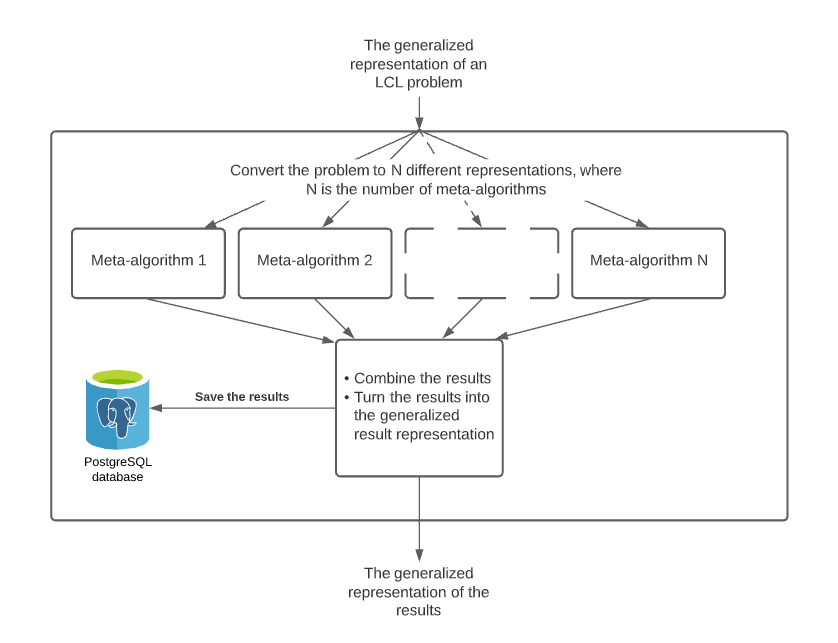
\includegraphics[width=\textwidth]{images/tool-architecture.png}
    \caption{High-level architecture of the implementation}
    \label{fig:implementation-architecture}
  \end{center}
\end{figure}

The database contains only three tables: one for
storing LCL problems together with their upper and
lower bounds, one for keeping track of what families of
problems have been generated and classified via batch
classification mechanisms, and one storing meta-data
of the meta-algorithms used in classifying the LCLs.
The front end is quite simple from technical perspective
too. Some of the details about the client side of the
application will be discussed more in Section~\ref{section:webinterface}.
The back end, however, contains most of the compplexity of
the tool. Therefore, in this section, we will concentrate
mainly on the sever side.

\subsection{Problem}

The core element of the whole application and of the
back-end part in particular is the Problem class.
For representing an LCL problem, we have decided
to use notation similar to that of Round
Eliminator. Our representaion however also
allows for graph types other than trees -- namely cycles.
Besides, it allows the underlying graph of a problem
to be rooted (or directed in the case of cycles).
Finally, it allows representing problems where
leaves' and root's output labels are also constrained.
The representaion similar to that of a Round
Eliminator has been chosen because of its generality.
In particular, as we have shown in Theorem~\ref{theorem:re_formalism_is_general},
any LCL problem
on $(\beta, \delta)$-biregular unrooted trees -- provided
that nodes of degrees other than $\beta$ and $\delta$ are unconstrained
and nodes near leaves are unconstrained -- can be represented
using the formalism used in the Round Eliminator.

Since we are only concerned with problems on regular trees and cycles
this representation works well for us. For the cases of cycles,
the only restriction is that degree of both passive and
active configurations has to be two. Also, the case
of directed (rooted) cycles (trees) can be handled
using the \emph{colon notation} that has been already
previously used in a recent paper on automating
the classification of LCLs in rooted trees~\cite{Balliu2021}.
Furthermore, the cases when \emph{irregular} nodes, i.e.
leaf nodes or root node, are restricted can also
be handled by specifying those restrictions
(separately for leaf nodes and a root node)
as separate properties of the Problem object.
Thus, our representation of LCL problems is general
enough to cover all the LCL problems that are
included in the scope of the project.

Having explained this, we can finally list all the
properties that are encapsulated into the
Problem object. The object contains the already
mentioned active configuration, passive configurations,
leaf constraints (which can be an empty set), root constraints
(which can be an empty set too), as well as special flag variables
indicating whether all active or all passive configurations
are allowed for active and passive nodes respectively.
If one of the two flag variables are set to true,
it overrides whatever is contained in the variables
holding the actual active and passive configs.
Besides, each problem object contains information
on the type of the underlhing graph: path, cycle or
tree. Notice that although any path is always a tree,
we chose to differentiate between those two
for convinience. It is worth mentioning that
a path graph type will be chosen as internal
representation whenever both active and
passive configurations are of degree two and
the user-selected graph type is not cycle.
In particular, if a user specifies tree as a graph
type and provides configurations of degree two,
tree will still be chosen as a graph type of the problem
internally. Finally, after parsing the configs
that are always provided in a string format,
the tool automatically decides whether the given problem's
underlyhing graph is rooted/directed or not.

It is also worth noting that as a first step of
creating a Problem object, the specified parameters,
including nodes' configurations and constraints
are checked for validity. Thus, if, for example,
a problem is misspecified so that some of the
configurations are "directed" while others are not,
an exception is thrown containing a message with
a human-readable explanation for why the
specification was invalid. After the validity
of the specification is checked, a problem is
normalized by executing the normalization algorithm
described below in Section~\ref{section:problem-normalization}.

\subsection{Classification}

Another central component of the back end is
the function responsible for classification of LCL problems.
On the high level, the function takes as input an LCL problem and
runs underlying meta-algorithms, some of which might be
able to provide some useful information about the complexity of the
problem. After that, the function combines the results
returned by all the meta-algorithms. Based on teh results returned,
the function determines the tightest known lower and upper bounds of
the LCL problem both in the deterministic and randomised LOCAL
models. Finally, a Response object is constructed based on the bounds
and is returned as the functions result. In the best case, tight
complexity bounds are found for both deterministic and randomized
settings. In the worst case, trivial bounds are returned:
"unsolvable" for upper bounds and $\Omega(1)$ for lower bounds.

Each of the underlying meta-algorithms or datasets is wrapped
in a function -- we will refer to it as "subclassify" from now on -- such
that it provides unified interface for the main
"classify" function. In particular, subclassify takes
as input an instance of the Problem class and
returns an instance of Response class. A Response object
simply encapsulates upper and lower bounds for both
deterministic and randomized settings. There is
exactly one subclassify function for each meta-algorithm
or dataset that we use. Inside each subclassify function,
we first check if the provided problem can be classified
at all by the underlyinng meta-algorithm. Often, we can
exit early already at this stage if, for examle, the meta-algorithm
in question deals only with rooted trees and the provided input is a 
problem on unrooted trees (or e.g. a problem on cycles). Then,
if we haven't exited the function yet,
we transform an instance of the Problem class to a problem
representation used by the meta-algorithm that the given
subclassify wraps around. The meta-algorithm is then executed,
the retured result is transformed into an instance of the
Response class and the Response object is returned as
a result of the subclassify function.

\subsection{Query}

The query class encapsulates some of the properties
based on which the database is queried for problems.
Only problems that satisfy the provided Query object will be
returned. The properties encapsulated by a Query object are
more or less directly mapped to an SQL query's WHERE clause.
The Query class groups those properties in three parent items:

\begin{itemize}
  \item problem properties,
  \item complexity bounds,
  \item include/exclude configuration.
\end{itemize}

\emph{Problem properties} define a class of problems that are to be
returned from the database. It includes the following fields:

\begin{itemize}
  \item active degree,
  \item passive degree,
  \item alphabet size (upper bound on it to be precise),
  \item Whether active/passive configurations are necessarily monochromatic,
  \item Whether underlyig graph directed/rooted or not,
  \item Type of the underlying graph. Which is always one of the following three
  options: tree, cycle, path.
\end{itemize}

\emph{Complexity bounds} limit the returned problems further by
restricting their complexities. The \emph{complexity bounds} object
contains the following items:

\begin{itemize}
  \item upper bound in randomized LOCAL setting (referred to as RUB),
  \item lower bound in randomized LOCAL setting (referred to as RLB),
  \item upper bound in deterministic LOCAL setting (referred to as DUB),
  \item lower bound in deterministic LOCAL setting (referred to as DLB).
\end{itemize}

The restriction of the fetched problems is done according to the
following logic: only those problems are returned (not filtered out)
whose known randomized upper bound is at most as high as RUB, whose
known randomized lower bound is at least as high as RLB, whose
known deterministic upper bound is at most as high as DUB and whose
known deterministic lower bounds is at least as high as DLB. Notice that
for a problem not to be filtered out, all the four criteria must be
satisfied.

Finally, \emph{include/exclude configuration} has the following
items encapsulated in it:

\begin{itemize}
  \item Whether only "smallest" problem has to be returned (in terms of the number of configurations).
  \item Whether only "largest" problem has to be returned (in terms of the number of configurations).
  \item Whether only those problems must be returned whose randomised upper
  and lower bounds do not match.
  \item Whether only those problems must be returned whose deterministic upper
  and lower bounds do not match.
  \item Whether only those problems must be returned whose randomised both
  upper and lower bounds are trivial (i.e. unsolvable and $\Omega(1)$
  respectively).
  \item Whether only those problems must be returned whose deterministic both
  upper and lower bounds are trivial (i.e. unsolvable and $\Omega(1)$
  respectively).
  \item List of configurations $L$ such that if a problem's configurations contain at least one configuration from $L$, the problem is excluded. Note
  the item has not effect if left empty.
  \item List of configurations $L$ such that if a problem's configurations contain all of the configuration from $L$, the problem is excluded. Note
  the item has not effect if left empty.
  \item List of configurations $L$ such that if a problem's configurations contain at least one configuration from $L$, the problem is included.
  Otherwise a problem is excluded.
  Note
  the item has not effect if left empty.
  \item List of configurations $L$ such that if a problem's configurations contain all of the configuration from $L$, the problem is included.
  Otherwise a problem is excluded.
  Note
  the item has not effect if left empty.
\end{itemize}

\section{Problem normalization}
\label{section:problem-normalization}

This section describes the above mentioned problem normalization
algorithm. The algorithm is used for determining which problems
are equivalent to each other. This, in turn, allows us
to reduce the amount of needed storage. Besides, this prevents
situtaions when a tool needs to run classification for a problem $A$
from the very beginning while an isomorphic problem $B$ has already been classified
by the tool previously and saved in the database. Thus, the normalization
algorithm also allows us to reduce the usage of computational resources.

The algorithm is based on the problem normalization algorithm
from Round Eliminator~\cite{Olivetti2020}. While the original
algorithm is written in Rust programming language, I
reimplemented it in Python and changed some of its
implementation details to better suit our purpose.
However, the general idea of the algorithm stays the same.

First, we determine how many labels are used in the description of the
problem $P$ i.e. its alphabet size. Then, we map each letter in the description
to a letter from A to Z. For example, if numbers were used for describing
the problem, the numbers will be mapped to capital letters of
English alphabet. It is important to point out already now that
one limitation of the current implementation is the fact that
a problem with more than 26 labels cannot be correctly normalized.
Once we obtain the list of letters used, we calculate all
permutations of the list. For each permutation, we execute the following
subroutine:

\begin{itemize}
  \item Based on the given permutation, create a mapping from each
  element of the problem's alphabet to each symbol in the permutation.
  That is, we map the $i$'th letter of the $P$ alphabet to the $i$'th symbol
  in the permutation for all $i$ from 1 to the size of $P$'s alphabet.
  \item Based on the obtained mapping, do the following with the problem's
  active configurations, passive configurations, leaf constraints and
  root constraints one at a time.
  
  \begin{itemize}
    \item For each line of the configurations/restrictions, rename symbols
    according to the mapping constructed above.
    \item If the problem $P$ is specified on unrooted/undirected graph,
    change position of all symbols on each line of the configurations/restrictions according to symbols alphabetical order.
    If the underlying graph of $P$ is directed/rooted, keep the currently first
    symbol as first, but change positions of all the rest symbols (again separately for each line)
    according to symbols alphabetical order.
    \item If at this point, some configuration lines are
    duplicated, remove all the duplicates so that each configuration
    line is unique.
    \item Sort the unique configuration lines in alphabetical order
    treating the lines as strings.
  \end{itemize}

  \item Return the newly constructed active configurations,
  passive configurations, leaf constraints and root constraints as
  a tuple of four elements.
\end{itemize}

Each execution of the subroutine described above yields a tuple
of size four. Thus, after executing the subroutine on each permutation of
labels, we eventually obtain a list of tuples of size four.
Then we sort the list, and take its first element. The four
tuple's elements are then assigned to the $P$'s
active configurations, passive configurations, leaf
constraints and root constraints respectively.

% \begin{algorithm}
% \DontPrintSemicolon
% \caption{\label{alg:normalize}normalize($P$)}
% \KwIn{problem $P$}
% \KwOut{problem $P$ with its constraints and configurations normalized}

% $lc \gets$ number of labels in $P$ \;
% $ls \gets$ first $lc$ capital letters of English alphabet \;
% $perms \gets$ a list of all permutations of $ls$  \;
% $all_normalized \gets$ empty array \;
% \For{every $perm$ in $perms$} {
%     add $normalizeForPermutation()$ $all_normalized \;
% }

% this is just an example 


% \Repeat{$R_{i} = R_{i-1}$}{
%   $i \gets i + 1$\;
%   $R_{i} \gets R_{i-1}$\;
  
  
% \uIf{$(\Sigma_\Pi,a \neq \epsilon) \in R_i$ and $\Pi$ is non-empty}{
%   \Return $\Sigma$
%   }
% \Else{
%   \Return $\epsilon$
% }
% \end{algorithm}


\section{Batch classification and reclassification}

This section describes how batch classification and
batch reclassification mechanisms have been implemented.
Batch classification is important since we want our database
to be prepopulated with significant number of classified
problems already before the first users start using it.
In particular, we would need to classify huge but finite
families of problems consisting of tens and hundreds of
thousands of LCL problems. Moreover, once a family of
problems is selected, the problems of the famnily need to
be generated and turned into instances of Problem class before
we can actually classify them. Batch reclassify functionality,
on the other hand, is needed for cases when, for one reason
or another, we would want to reclassify a certain
family of LCL problems that is already stored in our
database. For example, if we integrate a new meta-algorithm
to our solution in the future, we would need to reclassify
all problem families that are compatible with the newly-integrated
meta-algorithm. Or purhaps, a programming mistake has been
made when integrating one of the meta-algorithms, and therefore,
the problems need to be reclassified again.

One option for implementing batch reclassification
mechanisms would be to simply delete all of the problems
of the class in question from the database and execute
the batch classificatoin logic from the beginning
including its first step of generating the problems
of the problem class. However, this is suboptimal,
since generation of problems of a certain family
usually takes significantly longer times than
the subsequent classification step. For this reason,
we decided to have separate functionality for
batch reclassification.

The batch classification process starts with creating
an object that specifies a family of problems to be
generated, classified and stored in the database.
The specification includes properties like
active and passive degrees, label count, type of the
underlying graph, etc. The problems of the given
family are then generated via the following algorithm:

\begin{enumerate}
  \item Based on the specified label count, get a list of
  all symbols i.e. alphabet of the problem family
  \item Based on the alphabet and the specified active/passive
  degrees, generate lists of all the possible
  active and passive one-line configurations
  \item Get a list of all possible combinations
  of active one-line configurations and a list of all possible
  combinations of passive one-line configurations. The combinations
  can be of any size. This can be accomplished via
  the "powerset" function. Now we have lists of
  all possible active and passive configurations.
  \item Remove configurations that are empty.
  \item Generatate all possible tuples of size two
  where the first element is an active configuration and
  the second is a passive configuration. This corresponds
  to cartesian product between the previousy generated
  lists of all active and passive configurations.
  \item Remove tuples that have exact duplicates in the
  gnerated list of tuples, so that all tuples are unique.
  \item Turn each tuple into a Problem object using
  elements of the tuple as active and passive configurations.
  \item Normalize all the problems
  \item Now that all the problems are in a normalized 
  representation, it is easy to detect whether any two
  problems are isomorphic to each other. Remove such
  problems from the list so that the list contains only
  unique non-isomorphic problems.
  \item Return the list of newly-generated problems.
\end{enumerate}

Once the problems are generated, we store them to the database,
even though they are not classified yet. This is done mainly
because the database will automatically associate a unique
identifier with each of the problems.

After that, the problems are classified. Notice that
some of the meta-algorithms provide a way to classify
lists of problems at the same time, which is often
significantly faster than classifying one problem at a time.
This is due to the fact that some meta-algorithms
(e.g. TLP classifier and BRT classifier) are in fact
huge datasets of preclassified problems. When
classifying each problem individually, such
meta-algorithms would need to read out the whole
dataset from the disk, find one specific problem,
and return the result. On the other hand, when
classifying multiple problems at the same time,
numerous optimizations can be applied e.g. reading the 
dataset from the disk just once and search for all
requested problems at the same time. For this reason,
when batch classifying families of problems we first
call such batch classiicatio methods of meta-algorithm
if such methods exist. Once this is done, a modification
of the previously-described classify function is called
for each individual Problem object. The difference is
that if a meta-algorithm $A$'s batch classify method has been
already called, its "subclassify" function is not called
anymore during the individual-problem classification which
can significantly speedup the whole batch classification
functionality. Finally, when all problems have been classified,
the database is updated with the classification results.

The batch reclassification functionality resembles
what has been described above with the excpetion that,
once a family of problems has been specified, it is
not generated but is instead queries from the database.
After that, the fetched problems undergo the same
batch classification process. Finally, the database is
updated with the received classifications.

\section{Integration of Round Eliminator}

This section describes how the Round Eliminator
tool~\cite{Olivetti2020} has been integrated in our solution.
Prior to integration we had had considered several options:

\begin{itemize}
  \item Using an API of a server that runs the back end of the Round Eliminator tool
  \item Calling REtor as a command line tool from our Python
  application and then parsing the output, which is returned
  in a text format as part of stdout~\cite{stdio}
  \item Compiling REtor's source code to a "Shared Object" file (.so extension)
  using CPython ~\cite{CPython} bindings and then importing the compiled
  functions to our Python application as CPython dependency.
\end{itemize}

At the moment of writing the thesis, the Round Eliminator tool
is deployed using WASM~\cite{WASM}. This virtually means that
there is no back-end part running on a server, but instead
all of the logic is executed on the client side of the application.
Redeploying the tool with a standalone server and a separate client
part did not seem like a feasible alternative since this would
require a nontrivial amount of work from the tool's maintainers.
Thus, the first option was not feasible.

On the other hand, the second option was feasible. Indeed,
this method of using REtor had already been used in the
implementation of TLP Classifier~\cite{Rocher2020clas}. However,
this approach has several crucial disadvantages.
Firstly, the overhead of calling a command line command
from a Python program is significant compared to just calling
a Python function. Secondly, the output of Round Eliminator
would have to be parsed from the plain textual format, which
would have added an additional complexity of the software.
Finally, the approach complicates distribution and deployment of
the software. Indeed, one would have to install the specific
version of Rust programming language as well as download and
build form source codes the specific version of REtor required.

Instead, we have decided to go with the latter option. This
alternative does not have any of the disadvantages listed
in the previous paragraph while being just as feasible and
easy to implement. Compiled in this manner, the whole of
Round Eliminator logic is contained in a single .so file
that can be easily deployed to e.g. a production server.
Besides, the speed improvement is significant: we were
able to execute up to 3 rounds of round eliminator
in under 100 milliseconds. Finally, the functions
exposed via the .so file, return python-native
data structures so that no additional parsing is required on our side.
This, in turn has been achieved by adding CPythin bindings
to the REtor source code. The bindings wrap the relevant functions
written in Rust, thus enabling us to pass Python data structures
as parameters and recieve the return values as python-interpretable values.
The bindings were implemented using the rust-cpython library~\cite{RustCPython}.


\section{Web interface}
\label{section:webinterface}

This section will briefly discuss some implementation details of
the client side of the application. First, we start explaining why
the web interface has been implmented in the first place and why it
is important. Then, we describe some of the technologies that were
chosen as part of the implementation. Finally, we describe the
reasoning behind and advantages of the forms' state being stored
as a query part of the URL.

The reason why we decided to spend additional time and implement
the web interface can be best unnderstood when considering
another tool that has recently been rising in popularity among
the distributed algorithms community -- Round Eliminator~\cite{Olivetti2020}. The tool has proved to be a very useful utility
when doing research connected to LCL problems on biregular trees.
However, if it wasn't for the web interface that Olivetti has
implemented, it is most likely that the popularity and
frequency of use of the tool would have been nowhere near the current
levels. Indeed, almost all users of the tool use it via the web
client. Otherwise, a user would need to install Rust programming
language~\cite{Rust}, build the tool locally using the tool
called "Cargo"~\cite{Cargo} and then run it using the command-line.
It is clear that the number of people willing to do that would be
significantly smaller than number of people who ended up using
an easy-to-use web interface that requires no installation or 
configuration.

By analogy, we can assume with high confidence that significantly more
user would be willing to use our tool vie the web interface rather
than downloading the soource of the tool locally and installing
a specific version of Python programming language~\cite{CPython}.
Moreover, the richness of the web user interface allows us to convey complicated
ideas related distributed computing in way that is easier to understand, at least for knowledgable audience. Thus, it is has been
decided to spend some time resources -- even though they were 
quite limited -- on implementing a web user interface that is
relatively easy to use and understand compared to its
command line -based analog.

The web interface consists of two forms. One form for classifying
individual problems, and another one for issueing queries
about groups of problems against the database. When using the
first form, our application will first check if the requested
problem can be found in a database. If not, it will proceed to
running the classifiers (which corresponds with the "classify" function described above) and will eventially return the newly
classified result. If the classification result is not trivial (which means that lower bounds are constant and upper bounds are unsolvable),
it will also be stored in the database. The second "query" form, once
submitted will be transformed into the previously described
"Query" object. The query will then be executed against the database,
the results will be returned to the client side and rendered
in a user-friendly format.

As a programming language for our front-end application, we decided
to use TypeScript~\cite{TypeScript}. TypeScript is a general purpose
programming language developed and maintained by Microsoft. It is closely related to JavaScript programming language, which has become de facto standard programming language for the Web.
As a framework for our client application, we have decided to use
Svelte~\cite{Svelte}. Svelte is an open-source front-end framework
written in TypeScript. Among other things, it allows a simplified
approach for application state management, and reduces initial
page load times compared to other front-end frameworks~\cite{SvelteVsReactBundleSize}.

For the styling of the front end, we used a minimalist CSS framework
called "Milligram"~\cite{Milligram}. It provides a good starting point
when it comes to styling a modern web application. Besides, the total
size of the framework is just 2 kilobytes when zipped~\cite{Milligram}.
This, simplicity to use, and our previous positive experience with
the framework were the decisive factors that influenced our final
choice.

As a final interesting piece of technology used, we describe properties
and our reason for choosing to use svelte-virtual-list~\cite{svelte-virtual-list}.
The library allows rendering only part of the content instead of rendering
the whole of the content on a web page. In our case, this is
particularly useful as it allows us to
show tens of thousands of LCL problems (returned as part of the described above querying functionality) in a virtual list.
The virtual list, implemented via the above mentioned svelte-virtual-list library, renders only a small number (about 3--4)
LCL problems at the same time. At the same time, it allows user to
scroll through the list of problems with no noticable delay.
If not for the library, our client application would have to render
tens of thousands of LCL problems all at once. This would result in
the user interface freezing for a prologned period (up to several minutes).

Finally, we will explain the reasoning behind and benefits for
storing the state of the two forms as part of the URL's query
component. When searching for interesting query results, or even
just classifying different individual LCL problems, it is often
required to demonstrate the results to somebody else. To allow for such
a sharing, we decided to encode the state of both forms in the URL.
Thus, once e.g. the results of a query are obtained, it is possible
to copy the link and simply send it to, for example, a colleague.
When opening the link, both forms will be prefilled with
exactly the same values as those of the sender. This will make sure
that in most cases the sender and the reciever of the link will end
up with the same results displayed. Besides, if a particularly
interesting query has been discovered, it is possible to
simply copy and store the link. Opening the link in the future,
will prefill the forms with the same parameters and display
the same relevant results.

% \section{Deployment details}

% This section will outline some of the details related
% to how the application has been deployed. We will
% describe our high-level setup without listing all the
% details and configurations of each of the services used.

% We host our application on an infrastructure provided by
% CSC - IT Center for Science, Finland~\cite{FIXME}.
% The center provides an OpenStack solution, which is
% an open standard cloud computing software that provides
% infrastructure-as-a-service service. Our software
% is deployed to a virtual instance that was created
% via the OpenStack solution. The database is
% stored on a "volume", which unlike virtual instances,
% provide long-term persistent storage.

% FOr 


\chapter{Evaluation and further enhancements}
\label{chapter:evaluation}

In this chapter, I will attempt to evaluate success of the implementation
based on the research goals and the scope that I have outlined in Chapter~\ref{chapter:methods}.
Besides, I will also evaluate performance of the implementation.
As seen from the title,
I have decided to combine the evaluation with discussion on opportunities for further
development. Therefore, I will also propose several ideas for how my implementation
can be improved and extended.

\section{Decidability of a wide range of problem families on trees}

The first goal among the research goals listed in Chapter~\ref{chapter:methods}
was to store (or to be able to compute dynamically) most
(if not all) of the existing knowledge on classification of LCL problems on trees.
To evaluate how well I have done, we can refer once again to Table~\ref{table:summary}.
The first three columns under the ``Paths and cycles'' grouping refer to LCL problems on
paths and cycles where input is not allowed. The graphs can be directed or undirected,
have arbitrary (but finite) number of labels in the output, and have restrictions
on nodes of degree 1 (in cases of paths). All of these cases are covered by
the cycle-path classifier~\cite{Tereshchenko2020}, which is based on the recently
published paper~\cite{Chang2020}. The classifier has been integrated into the
solution and, thus, I claim that the problems of this family are fully classifiable by the tool.
The forth column of the table refers to LCL problems on paths and cycles
where input labeling is allowed. Since none of the used classifiers
are capable of processing problems with inputs, this family of problems
has not been covered by my implementation, although it has been shown that
LCLs of this class are decidable (even though it is PSPACE-hard)~\cite{Balliu2018}.

As can be seen from the first column of the ``Tree'' grouping, it is unknown whether
unlabeled regular homogeneous~\cite{BalliuHomogeneous}
undirected trees are classifiable if the number of
output labels exceeds two. On the other hand, LCL problems on
unlabeled regular undirected trees with binary label output is fully decidable, albeit
only in deterministic setting. In addition to this, for some problems of the problem family,
complexity is decidable even in randomised setting~\cite{Balliu2019c}.
Since my solution does not directly include a classifier that would implement
classification of problems of the described family, the tool is not capable of
classifying the problems. It is important to notice however that the TLP
Classifier~\cite{Rocher2020clas} uses the classifier as part of its implementation.
Therefore, at least some problems of the described family can be classified. Specifically,
only problems on (2, 2)-, (2, 3)-, and (3, 2)-biregular trees of the family
(and only in deterministic setting) can be classified in my implementation.
Therefore, a natural opportunity for extending the current functionality of the tool
would be to integrate a clasifier that would classify all binary labeling LCL problems
on unlabeled regular undirected trees. Given that such implementation would
essentially involve a simple table lookup (the authors of the original paper
reduce the classification problem to a two-dimensional table lookup), the
classifier could work efficiently even with trees of relatively high degree.

The next column in the table is for LCL problems on unlabeled regular directed
trees. It has been shown that the problems of this family are fully decidable
with any finite number of output labels~\cite{Balliu2021}. However, the
only currently-existing implementation of the decidability algorithm
works exclusively with binary rooted trees~\cite{Studeny2021}. The
meta-algorithm has been successfully integrated into the solution, and
thus all LCL problems on binary rooted trees can be classified also in
practice using the tool. Nevertheless, an implementation of the
decidability algorithm that would work for trees of higher degrees
would be of high interest to the research community. The original
paper shows that such implementation for arbitrary number of output
labels is possible at least in principle. Besides, there is no
evidence that such implementation would be impractical from the
performance perspective. Therefore, a natural opportunity for
extending the software would be to build such an implementation and
consequently integrate it into the tool.

All other -- more general -- LCL problem families
are currently only known to be decidable between complexity classes of
$\Omega(\log n)$ and $O(n)$~\cite{Chang2020a}. There are currently
no known implementation of the classification algorithm described in the
referenced paper. Although the described meta-algorithm is at least
EXPTIME-hard, there is also no evidence that the algorithm would not be
practical at least for a limited subfamily of problems. Therefore, its
implementation and integration into my solution would be a potential
direction for the tool's future development.

Thus, while many of the listed graph families are already classifiable
with the tool, more meta-algorithms can be developed
and integrated. Moreover, the theoretical
research of decidability of LCL problems on tree is currently
developing at a high pace, which will likely bring even more
positive theoretical decidability results in the future.
It is then the task of the practitioners to catch up with
the theory and make the practical decidability landscape
as complete as possible.

\section{Finding a problem's complexity and performing group queries}

The two other goals in the list of the research goals were

\begin{enumerate}
  \item to be able to find deterministic and randomised complexity of
  of a particular problem $P$, provided that the problem belongs to
  one of the classes that the tool is capable of classifying,
  \item to be able to query for groups of multiple problems based
  on a variety of parameters.
\end{enumerate}

As can be seen from Chapter~\ref{chapter:implementation},
both of these functionalities have been succesfully implemented.
Notice that
I address performance issues in another section later in
this chapter. Also,
I have already evaluated the number of
problem families the tool is capable of working with. In this section,
we are discussing just the availability of the functionality itself, while not
being concerned with other, although related, metrics.

% Finding out complexity of a specific problem takes consistently under
% 2 seconds, and performing a query might take from as little as several milliseconds
% in some cases to several seconds in most cases
% up to just under 35 seconds in rare cases when the volume of the queried data is particularly large.
% Notice that the rough performance results presented above are as measured
% from the perspective of the Web interface user, and thus include
% network delay as well as time it takes for the front-end logic to process
% and render the results.
% Thus, we can conclude that the two goals have been fully accomplished.

As a final research goal in the list, we had a possibility
to see which of the meta-algorithms has determined each
of the lower and upper bounds for each of the preclassified
LCL problems being stored in the database. As described in the
previous chapter, this is automatically done for all problems being
classified via my solution. At the same time as a problem is classified,
all of its classification results --- deterministic upper bound,
deterministic lower bound, randomized upper bound, randomized lower bound --
are associated with one of the meta-algorithms. This information is also
persisted in the database at the same time a newly classified problem
is being stored. Thus, we can consider this research goal as being
fulfilled as well.

\section{Performance}

In this section, we will evaluate my implementation from
performance perspective. Performance is essential for
the tool to be useful for the research community.
We will evaluate performance of the tool
in the context of classifying a single LCL problem and
querying the database for a group
of problems matching user-defined specification.

Notice that the purpose of this section is to evaluate how
useable the tool is from the perspective of its users.
Therefore, we are not concerned with exact millisecond
precision of the operations. Instead, I will present
the performance results with the precision down to a tenth of a second.
Notice also that the times will vary depending on the underlying
hardware, the fact whether other users are using the tool at the same
time, etc. All the results presented below are performed on the
author's local machine (MacBook Pro, 13-inch, 2018, Four Thunderbolt 3 ports).
Refer to the technical specification on the Internet for exact
hardware specifications of the machine.

Finally, when presenting results for classifying a problem or
performing a query, I measure the time it takes
for the corresponding function to execute as defined in the back-end
part of the implementation. Therefore, the time as experienced by the users of
the Web interface might be somewhat longer since it would include
also a network delay and executing front-end logic.

\subsection{Classifying a problem}

If a requested problem already exists in the database, finding out
the problem's complexity consistently takes less than a second.
On the other hand, if a problem has to be classified dynamically,
classifying it will take less than 3.2 seconds (at least in case when
problems degrees are less than 5 and the number of labels allowed is less
than 5 as well). Below are some of the performance measurement results,
based on which the above-mentioned conclusions has been drawn.

\begin{itemize}
  \item Any 2-labeling problem on undirected paths is classified in \emph{under 0.1 sec.}
  \item Any 3-labeling problem on directed (3, 2)-biregular trees is classified in \emph{under 0.7 sec.}
  \item Any 3-labeling problem on undirected (3, 2)-biregular trees where passive configurations are monochromatic is classified in \emph{under 3.2 sec.}
\end{itemize}

\subsection{Querying a problem family}

Below is a similar list of performance results for the querying
functionality. The query that retrieves the largest problem class, in terms of
number of problems, takes under 20 seconds. Notice that this query
finds and fetches several tens of thousands of problems. Queries
that fetch only a couple of hundred of problems are executed in under 1.5 seconds.

\begin{itemize}
  \item All 2-labeling problem on undirected paths are fetched in \emph{under 0.2 sec.}
  \item All 3-labeling problem on directed paths are fetched in \emph{under 7.7 sec.}
  \item All 3-labeling problem on directed (3, 2)-biregular trees are fetched in \emph{under 20 sec.}
  \item All 3-labeling problem on directed (3, 2)-biregular trees where passive configurations are monochromatic are fetched in \emph{under 0.3 sec.}
  \item Any 3-labeling problem on undirected (3, 2)-biregular trees where passive configurations are monochromatic are fetched in \emph{under 3.2 sec.}
  \item Any 3-labeling problem on undirected (3, 2)-biregular trees where active configurations are monochromatic are fetched in \emph{under 1.1 sec.}
\end{itemize}

Based on all the obtained performance results, as
well as based on the feedback that I have received
from the members of the research community who
already used the tool, it is
evident that the performance is fast enough for the
tool to be useful for the kinds of tasks it is intended for.
On the other hand, waiting for more than 20 seconds might prove
to be impractical or at the very least inconvinient
in many case. Therefore, improving the
performance -- especially
the performance of the querying functionality -- is
a natural improvement direction that would most
likely provide a lot of value for the users of the solution.

\section{Number of preclassified problems}

At the moment of writing the thesis, the database contains $335\,314$
LCL problems. Out of them, $197\,218$ have at least one non-trivial bound. \emph{Trivial bound} here
refers to $\Omega(1)$ for lower bounds and \emph{unsolvable} for upper bounds.

The following families of LCL groups have been pre-generated and batch classified
using the batch classification functionality described in Chapter~\ref{chapter:implementation}:

\begin{itemize}
  \item binary labeling problems on both directed and undericted paths and cycles,
  \item ternary labeling problems on both directed and undirected paths,
  \item 4-labeling problems on undirected paths,
  \item binary labeling problems on both rooted and unrooted (3, 2)-biregular trees,
  \item ternary labeling problems on unrooted (3, 2)-biregular trees,
  \item ternary labeling problems on rooted (3, 2)-biregular trees where passive configurations are monochromatic,
  \item 4-labeling problems on rooted (3, 2)-biregular trees where active configurations are monochromatic,
  \item a part of 4-labeling problems on directed paths,
  \item a part of ternary labeling problems on rooted (3, 2)-biregular trees (with no constraints on active or passive configurations),
  \item a part of 4-labeling problems on rooted (3, 2)-biregular trees where passive configurations are monochromatic.
\end{itemize}
Notice that in all of the problem families listed above, leaf and root nodes
(or equivalently nodes of degree one on paths) are unconstrained. Moreover, in addition to the
groups of preclassified problems, the database contains several individual problems that
were added as a result of the application being used by several of the members of the
distributed algorithms research community.

Thus, it is evident that the number of preclassified problems is already at this stage sufficient
for the tool to be useful to the research community.
On the other hand, all of the problems currently stored in the database are such
that the number of the allowed labels is limited to under 5 and degrees of the nodes
are limited to under 4. This is a huge limitation, and it would be
highly useful to investigate ways in which it can be mitigated.
Therefore, populating the database
with more problems of more diverse problem families is a natural opportunity for future
development.

\section{Miscellaneous}

This section contains some of the possibilities
for improving and extending the solution. The ideas collected
here has been obtained as a result of feedback
received from members of the distributed algorithms
research community who had already used the system
as part of their research process.

Currently, it is only possible to specify an upper bound for
the number of labels used in a problem when constructing a query.
A common request was to also be able to specify a lower bound for the
number of labels.

Another request was the ability to query only for those problems that are
or lead to periodic points as a result of applying round elimination.
The information about whether a problem is a periodic point ot not
is currently only available at the time of classification but is
not stored in the database. Storing the data and allowing for
querying based on it would be yet another possibility to expand the tool.

Similarly, it would be useful to query for problems based on their
exact constant complexity (as opposed to asymptotics) if such
information is available. Besides, displaying precise constant complexity
would also be benefitial when classifying a single problem.
Currently, precise constant complexity is sometimes available when
classifying a problem with the Round Eliminator. Storing this
information to the database, showing it to users and incorporating it
in the Query object would be another useful extension to the tool.

Finally, the query functionality is still currently rather limited.
Moreover, it is not clear which features of it are going to be the
most useful to the users and which will not be used often.
Thus, investigating this via collecting feedback from
research community and then modifying the tool based on
this feedback is yet another opportunity for improving the software.


 
\chapter{Conclusions}
\label{chapter:conclusions}

Time to wrap it up!  Write down the most important findings from your
work.  Like the introduction, this chapter is not very long.  One to
two (never over three) pages might be a good limit. Still, the chapter
gives the background, goals, content, and the findings. However, all that
should already be in the previous chapters. This is just a summary (as
are the abstract and the introduction).

For making PDF/A version requested by the Aalto Library, open the end result pdf file in Acrobat and store it as PDF/A. Then verify the result (everything should be fine, at least as PDF/A-2b version works).

Congratulations, your thesis is ready and it looks beautiful!



% Load the bibliographic references
% ------------------------------------------------------------------
% You can use several .bib files:
% \bibliography{thesis_sources,ietf_sources}
\bibliography{sources}


% Appendices go here
% ------------------------------------------------------------------
% If you do not have appendices, comment out the following lines
% \appendix
% \chapter{First appendix}
\label{chapter:first-appendix}

This is the first appendix. You could put some test images or verbose data in an
appendix, if there is too much data to fit in the actual text nicely.

For now, the Aalto logo variants are shown in Figure~\ref{fig:aaltologo}.

\begin{figure}
\begin{center}
\subfigure[In English]{
\includegraphics[width=.8\textwidth]{images/aalto-logo-en}}
\subfigure[Suomeksi]{
\includegraphics[width=.8\textwidth]{images/aalto-logo-fi}}
\subfigure[På svenska]{
\includegraphics[width=.8\textwidth]{images/aalto-logo-se}}
\caption{Aalto logo variants}
\label{fig:aaltologo}
\end{center}
\end{figure}


% End of document!
% ------------------------------------------------------------------
% The LastPage package automatically places a label on the last page.
% That works better than placing a label here manually, because the
% label might not go to the actual last page, if LaTeX needs to place
% floats (that is, figures, tables, and such) to the end of the 
% document.

\end{document}
